% !Mode:: "Tex:UTF-8"
\chapter{解空间投影等价的混淆算法}
\label{chap:4}

\section{引言}%
在第三章中,假设攻击者仅仅会从分析CNF公式入手,获取结构信息。
针对上述攻击模式,提出了CNF 公式结构隐私保护的的混淆算法。

而在本章中,将在前一章工作的基础上再进一步,
假设攻击者已经确切知道公式中夹杂了噪音变量和子句,
因而试图从分析解的角度出发,还原CNF公式,而后再获取其中携带的结构信息。

本章针对上述的隐私保护威胁,对“解空间投影等价的混淆算法”进行了深入的研究。
通过引入具有簇形解的噪音CNF 公式,
使噪音变量的取值不再唯一,
消除攻击者利用ALLSAT还原CNF 公式的可能性,
从而实现结构信息的隐私保护。

\section{问题描述}
第三章提出的CNF混淆算法,通过在原始CNF公式中混入仅有唯一解的噪音CNF,在隐藏原有CNF 携带的结构信息的同时,还保证混淆前后的解空间等价。
混入唯一解的噪音CNF,也就意味着在混淆后的解中,这些噪音变量都将只有唯一的取值。
从解混淆攻击者的角度看,对混淆后CNF公式的攻击破解点之一,就是寻找出赋值唯一的噪音变量。
一旦确认噪音变量,就可能将按照嵌入规则添加到原始子句中的额外文字取出,恢复原有子句,进而获得原始的CNF 公式,并取得其中的结构信息。

在详细描述之前,先介绍与之相关的术语。
\subsection{ALLSAT求解}
多数SAT问题具有一个以上的解,求解出SAT问题所有解的过程称为ALLSAT求解。
直观上看,调用一次SAT求解器可以获得SAT的一个解。
将已知解中每一个变量的赋值求反,以获得其反文字,并将所有这样的反文字的合取作为阻断(block)子句并加入到待求解的SAT 问题公式中,以引导求解器避开已搜索过的解。
通过多次重复,最终可以获得SAT问题所有的解。

本文中给出基于Craig插值\upcite{InterpBoolFunction,DBLP:journals/jsyml/Craig57} 的求解算法。
Craig插值是一阶逻辑定理证明中的一个强大工具。
为了简明起见,在这里将仅讨论命题逻辑中的Craig插值。
Craig插值的定义是,对于两个命题逻辑公式$F_1$和$F_2$,假设他们的支撑集(输入变量集合)为$V_1$和$V_2$,
且有$F_1\wedge F_2$不可满足,则存在$F_3$,使得$F_1\rightarrow F_3$成立,$F_3\wedgeF_2$不可满足,且$F_3$的支撑集为$V_1\cap V_2$。
很显然,$F_3$是$F_1$的一个抽象,既包含了$F_1$的所有情形,又具有更少的支撑集变量。
$F_3$就是一个Craig插值。
%因此,Craig插值于2003年开始成为自动构造抽象模型的强大工具[30]。
%从2007年开始,大部分的逻辑综合算法又都找到了基于Craig插值的高效实现,如函数相关性[47]、 逻辑分解[53][54]、特征化[41]、增量修正[55]和布尔函数匹配[56]。因此,Craig插值已经成为基于SAT的推理工具的另一个强大推理引擎。

使用Craig插值的最常用和最高效算法是McMillian算法\upcite{interp_McMillan}:首先构造两个相互矛盾的公式,
然后使用SAT求解器得到他们的不可满足证明,
然后使用定义\ref{def_gencraig}所描述的方法,
从不可满足证明中抽取Craig 插值。
而在文献\upcite{interpNoProof}中,
Craig插值的产生过程类似于传统的可满足赋值遍历算法。
不过其扩展算法包含两步,
分别对应于两个参与计算的公式。
该算法不需要产生不可满足证明的Craig插值算法。

\subsection{基于ALLSAT求解和分区的攻击}
根据前一章给出的CNF公式混淆算法,可知其中Husk变量的赋值是唯一的。
根据SAT问题的特点可知,对混淆后的CNF公式进行ALLSAT求解,可以得到混淆后公式的全部解。
因此,攻击者可以从中筛选出赋值唯一的变量。
由于原始CNF中也可能存在其他赋值唯一的变量,例如用于属性验证时的属性变量;
因此这些具有唯一赋值的变量可作为Husk变量的候选者;
攻击者可以通过构建仅包含这些唯一赋值变量的分区\upcite{Partition},
来获取Husk公式,并识别出Husk变量,从而恢复出原始公式。

假设Husk变量的个数是$m$,
原公式中取唯一赋值的变量数是$n$,
完全找出$m$的概率为$1/{C_{m+n}^m}$。	
由于原始公式中的$n$值一般为待验证属性变量,
当$n$值较小时,
解混淆攻击成功的概率将会变得很大。
因此必须解决上述问题。



\section{解空间投影等价的混淆算法}
%\subsection{设计目标}
%When we design the Cloud or grid oriented SAT solving framework, the following four goals are taken into consideration:
本章所给出的混淆算法,在设计时,考虑下面四个因素:

\begin{enumerate}
 \item
%First,
可移植性:目前的SAT求解器集成了冲突检测\upcite{EFFCON}等高效求解机制,因此希望可以将其作为黑盒直接使用,而不是像文献\upcite{OBfuscationd-CNFs}试图使用新的求解算法。
 \item \label{4:g2}
隐形性\upcite{obfuscationBible}:混淆算法可以保证电路结构信息无法通过对CNF公式的分析来获取。
\item \label{4:g3}
适应性\upcite{obfuscationBible}:求解框架应能防止第三方通过ALLSAT 来获取求解结果,进而识别出噪音变量。
 \item
开销:混淆算法不应该引入太多的开销。
\end{enumerate}
%\subsection{解空间投影等价}

根据上述目标,
为了保持混淆后的CNF公式对求解计算的透明性,
根据第\ref{chap:3}章中给出的SSH规则对原始CNF公式进行混淆,
在CNF公式的子句中加入新的文字,并在公式中加入新的子句。
新加入的文字和一部分新的子句来自于具有特殊解形式的可满足CNF公式,这个公式称为簇形Husks公式。
SSH规则保证原始的CNF公式可以和簇形Husks公式无缝地混合在一起,以便于达到\ref{4:g2}) 和 \ref{4:g3}) 的要求。
SSH规则在第\ref{chap:3}章中已经给出定义,出于本章叙述的完整性,
在本章的小节\textit{\ref{4:embeded rules}}中仍旧会给出详细的定义。

\begin{definition}[簇形解]\label{4:Cubic-Husk-Solution-definition}
假设CNF公式有$m+n$个变量,且$m$和$n$均大于0。
公式有$k$个可满足解。
其中$n$个变量的赋值在$k$ 个解中都相同,
另外$m$个变量的赋值在$k$个解中不全相同。
部分变量具有完全相同赋值的这$k$个解就构成一个簇形解。
\end{definition}

\begin{definition}[簇形Husks 公式]\label{4:Cubic-Husk-formula-definition}
Husk公式是有簇形可满足解的CNF公式,并且解变量的赋值是非特异的(不是全0或全1)。
\end{definition}


与第三章相同,
基于混淆算法的SAT求解隐私保护框架包含$GENERATOR$, $OBFUSCATOR$, $MAPPER$ 和 $VERIFIER$ 算法,
除了$GENERATOR$,
其余算法和第三章相同。
新的$GENERATOR$在\ref{4:genhusk}节介绍。

\subsection{簇形Husk公式的产生}\label{4:genhusk}
产生可满足CNF公式的算法有多种\upcite{microgenSAT,genSAT}。
本章中,定义\ref{4:Cubic-Husk-formula-definition} 中指出的簇形Husks公式采用质因数的方法构造\upcite{genSAT}。
如算法\ref{4:algo2_gen}所示。


\begin{algorithm*}[b]
\caption{$GENERATOR$}
\label{4:algo2_gen}
\begin{algorithmic}[1]
%%\SetAlgoLined
%\SetAlgoNoLine
\STATE input : NULL
\STATE output : Husks CNF $F_H$ and Husks result $R_H$
\STATE Generating prime numbers $p_A$ and $p_B$  ; \label{4:primenumber}
\STATE $\Phi= M(I_1 \neq 1, I_2\neq 1, O=p_A*p_B)$ ;\label{4:multiplePrime}
\STATE $F_H=Tseitin(\Phi)$ ;\label{4:TseitinPHI}
\STATE $R_H=\{a_{i_j}|1\le i_j\le n,a_{i_j}\equiv b_{i_j}\}$ ;
\end{algorithmic}
\end{algorithm*}

%产生Husks公式的GENERATOR的实现在算法一\ref{4:algo2_gen}中描述。
%%
%\textbf{First},
%given two primes $p_A \neq p_B$ (at line \ref{4:primenumber}),
%% represented by a binary vector $p_A = <a_1,a_2,\dots,a_n>$, $p_B = <b_1,b_2,\dots,b_n>$,
%we assign $p_A \cdot p_B$ to the output of a multiplier $M$ with constraint $I_1\ne 1$ and  $I_2\ne 1$ (at line \ref{4:multiplePrime}).
%$I_1$ and $I_2$ are inputs of $M$.
%
%\textbf{Second},
%we convert the multiplier $M$ into CNF formula $Tseitin(M)$ (at line \ref{4:TseitinPHI}).

\begin{enumerate}
\item \textbf{首先},
给定两个质数$p_A \neq p_B$(第 \ref{4:primenumber} 行),且两者具有如下的关系:
其二进制向量表示为$p_A=<a_1,\dots,a_{n+m}>$和
$p_B=<b_1,\dots,b_{n+m}>$。
% represented by a binary vector $p_A = <a_1,a_2,\dots,a_n>$, $p_B = <b_1,b_2,\dots,b_n>$,
将$p_A * p_B$ 赋值给乘法器$M$的输出,并且限制$I_1\ne 1$ and  $I_2\ne 1$ (第\ref{4:multiplePrime}行)。
其中,$I_1$和$I_2$ 是$M$的输入。

\item \textbf{其次},
将乘法器$M$编码为CNF公式$Tseitin(M)$(第\ref{4:TseitinPHI}行)。
\end{enumerate}

为了满足$Tseitin(M)$,
$M$的两个输入一定是$\{I_1=p_A,I_2=p_B\}$ 或者 $\{I_1=p_B,I_2=p_A\}$。
根据条件两个解具有部分相同的赋值,
即存在$n$个正整数下标$\{i_j|1\le j\le n\}$,
其中每个都满足$1\le i_j\le n$,
使得$a_{i_j}\equiv b_{i_j}$。
直观的,
$\{i_j|1\le j\le n\}$是具有相同取值的$a_{i_j}$和$b_{i_j}$的下标$i_j$的集合。
令$R_H=\{a_{i_j}|1\le i_j\le n,a_{i_j}\equiv b_{i_j}\}$。
$R_H$也称为该公式的簇形解公共赋值变量集。



\subsection{解空间投影等价的混淆}\label{4:obfuscating}

为了防止CNF公式以及解的信息泄露,给出了一个隐私保护的策略。
该策略基于下面的事实和期望:
\\$\textbf{事实 1:}$ 改变公式中的CNF标记和关键子句,可以使基于模式匹配或子图同构的电路结构恢复技术失效。
\\$\textbf{事实 2:}$ 混淆后的解空间不应该被缩小,否则会误导真实应用,例如验证等。
\\$\textbf{期望 1:}$ 鉴于事实2, 解空间可以被扩大,以便于误导公共云上包括SAT求解器在内的第三方。
\\$\textbf{期望 2:}$ 可以通过投影的方式,从混淆后公式的解中较快的恢复出原始公式的解。

本文给出的隐私保护算法,称为$OBFUSCATOR$。
该算法使用解空间投影等价算法,
将Husks公式$F_H$嵌入到原始公式$F_C$中,
产生一个新的CNF公式$F_O$。
$OBFUSCATOR$改变子句的文字集合以及公式中的子句集合,
来防止公式中的电路结构被恢复。
通过SSH规则混淆后,原公式解空间被成倍数扩展,
以防止在公共云上的SAT求解器获取原始公式的解。
其中倍数为簇形解公式的解个数,
并且原始公式的解可以通过投影的方式从混淆后公式的解中获取。

\subsubsection{解空间投影等价(SSPE)算法}\label{4:embeded rules}

让我们在第\ref{chap:3}章的基础之上,考虑一个更复杂一些的问题:
将SAT问题编码为CNF公式外包到云中,由SAT 求解器求解;
并且不希望SAT求解器知道原始公式以及它的解的个数。

一个简单的方法是:
将原始的CNF公式,
和具有多个解,且和原始公式无共同变量的可满足公式
混合在一起,并将混合后的CNF 公式外包的云上。
原始公式的解将会混杂在混合公式的解中,
并且解的个数为两个CNF公式解的个数的乘积。
但是,这种简单混合的可识别性很高,
基于分区\upcite{Partition}的方法可以将两个不相关的公式分离开来,
从而得到原始的CNF公式。

一个改进的方法是:
对任意公式$F_C$,
产生一个可满足公式$F_H$及其一个解$R_H$。
$F_C$和$F_H$没有公共变量,也即:$V_{F_C}\cap V_{F_H}\equiv \phi$。
我们将采用如第\ref{chap:3}章所给出的方法,
将$F_C$和$F_H$无缝混合,
以便于隐藏$F_C$。
同时,
保持$F_C$中的所有解都包含在新的公式中。

为实现$F_C$和$F_H$无缝混合,
直觉的方法是将$F_H$中的变量加入到$F_C$的子句中,
并且使用$F_C$和$F_H$中的变量产生新的子句。
由于CNF特性,
导致对任何CNF公式$F_C$,
在其子句中加入新的文字可能会扩展解空间,
而加入包含$F_C$中变量的子句则会缩减解空间。
那我们如何在此情况下保证$F_C$所有的解仍旧保留在新的公式中,
并且新公式的解空间在原始变量上的投影和原始解空间完全等价。
在给出具体答案之前,首先澄清下面的概念。

\begin{definition}[解包含关系 $S_C \subseteq S_O$]~
CNF 式$F_C$和$F_O$具有$n_{F_C}$个公共变量$x_1,...,x_{n_{F_C}}$ 。
并且有
$|V_{F_C}|\equiv n_{F_C}$,$|V_{F_O}|\equiv n_{F_O}$,
且$ n_{F_O}\geqslant n_{F_C} > 0$。
$S_C$和$S_O$分别是$F_C$和$F_O$的解。
在$S_C$和$S_O$中,$n_{F_C}$ 个公共变量的赋值是相同的,
即对任何$1\le i\le n_{F_C}$,
有$S_C(x_i)\equiv S_O(x_i)$。
我们称解$S_C$包含于$S_O$,
记为$S_C\subseteq S_O$。
\end{definition}

%\begin{definition}[解空间等价(SSE)]\label{4:SSEdefinition}~
%CNF公式$F_C$有$n$个解$\{S_{C_1},...,S_{C_n}\}$;
%CNF公式$F_O$也有$n$个解$\{S_{O_1},...,S_{O_n}\}$,
%并且对于任意$i \in [1,n]$, $S_{C_i} \subseteq S_{O_i}$。
%我们称$F_O$解空间等价于$F_C$,记为$F_C \equiv_{_{SSE}} F_O$。
%\end{definition}

\begin{definition}[解空间投影等价(SSPE)]\label{4:SSPEdefinition}~
CNF公式$F_C$有$n$个解$\{S_{C_1},...,S_{C_n}\}$。
CNF公式$F_O$有$n * m$个解$\{S_{O_1},...,S_{O_{n \cdot m}}\}$。
对于任意$1\le i\le n$和$0\le j\le m-1$,
有$S_{C_i} \subseteq S_{O_{i + {n * j}}}$,
则称$F_O$解空间投影等价于$F_C$,
记为$F_C \equiv_{_{SSPE}} F_O$。
\end{definition}

%\begin{definition}[解空间上估计(SSO)]\label{4:SSOdefinition}~
%CNF公式$F_C$有$n$个解$\{S_{C_1},...,S_{C_n}\}$;
%CNF公式$F_O$,
%有$m$个解, $\{S_{O_1},...,S_{O_n},...,S_{O_m}\}$,
%并且$m \geqslant n$,
%并且对于任意$i \in [1,n]$, $S_{C_i} \subseteq S_{O_i}$。
%我们称$F_O$ 的解空间是$F_C$ 的上估计,记为$F_C \vdash_{_{SSO}} F_O$。
%\end{definition}
为了在新公式中保持$F_C$公式中的所有解,
仍然需要使用第\ref{chap:3}章提出的解空间保持(SSH)规则。
与第\ref{chap:3}章不同的是,
本章使用公式$F_H$和其簇形解的公共赋值变量集合$R_H$来混淆公式$F_C$,
以便于保证混淆后公式具有投影等价的解空间。

%\textbf{解空间保持(SSH)规则: }
%\begin{enumerate}
%\item \textbf{规则 1}:
%对任一子句$c\in F_{C}$,
%从$R_H$中任取出变量,
%并按照下列规则插入到子句$c$:
%如果在$R_H$中变量的赋值是$T$,作为负文字;
%如果在$R_H$中变量的赋值是$F$,作为正文字;
%用新生成的子句代替原始子句$c$。
%\item \textbf{规则 2}:
%%generating new clauses with literals from $R_H$ and output variables in $F_C$ according to the following rule:
%使用$R_H$中的文字和$F_C$中的变量创建新的子句,按照下列规则:
%如果在$R_H$中文字是$T$,就作为正文字;
%如果在$R_H$中文字是$F$,就作为负文字。
%Literal of output variable is extracted directly from the key clause and inverted.
%\end{enumerate}
%
%\begin{definition}[${\textbf{Obf(}}F_C,F_H,R_H\textbf{)}$]\label{4:OBFUSCATORSSH}
%For arbitrary formula $F_C$, and satisfiable formula $F_H$ with $R_H$ as one of its assignments,
%$Obf(F_C,F_H,R_H)$ is the result of applying SSH Rules when blending $F_C$ with $F_H$.
%If $F_H$ is a Singular Husk formula and $R_H$ is its unique solution, $Obf(F_C,F_H,R_H)$ is called ${\textbf{SSE obfuscation}}$.
%If $F_H$ is Husks formula and $R_H$ is one of its solutions, $Obf(F_C,F_H,R_H)$ is called ${\textbf{SSO obfuscation}}$。
%\end{definition}

\begin{definition}[${\textbf{Obf(}}F_C,F_H,R_H\textbf{)}$]\label{4:OBFUSCATORSSH}
对任意公式$F_C$,
和可满足公式$F_H$及其一个部分赋值$R_H$,
$Obf(F_C,F_H,R_H)$ 是在基于SSH规则将$F_C$和$F_H$混合后得到的公式。
%如果$f_h$是单一hUSK公式并且$r_h$是它的唯一解, 就称$oBF(f_c,f_h,r_h)$为${\TEXTBF{sse OBFUSCATION}}$。
如果$F_H$是簇形Husks公式,
并且$R_H$是其簇形解公共赋值变量集合,
就称$Obf(F_C,F_H,R_H)$ 为${\textbf{SSPE 混淆}}$。
\end{definition}
% \begin{definition}[${\textbf{Obf(}}F_C,F_H,R_H\textbf{)}$]\label{4:OBFUSCATORSSH}
% For arbitrary formula $F_C$, and satisfiable formula $F_H$ with $R_H$ as one of its solutions,
% $Obf(F_C,F_H,R_H)$ is the result of applying SSH Rules when blending $F_C$ with $F_H$.
% If $F_H$ is a Singular Husk formula, $Obf(F_C,F_H,R_H)$ is called ${\textbf{SSE obfuscation}}$.
% If $F_H$ is Husks formula, $Obf(F_C,F_H,R_H)$ is called ${\textbf{SSO obfuscation}}$.
% \end{definition}

%For SSH based obfuscation, we have following theorems.
对SSPE混淆,下列定理成立。

%\begin{theorem}[SPE Obfuscation]\label{4:SSEtheorem}
%
%对任意CNF公式 $F_C$,和单一Husk公式$F_{_SH}$,如果
%
%~~$V_{F_C}$ $\cap$ $V_{F_{_SH}}$ =$\phi$, 并且
%$R_{_SH}$是$F_{_SH}$的唯一解,
%
%则 $Obf(F_C,F_{_SH},R_{_SH}) \equiv F_C\wedge F_{_SH}$。
%\end{theorem}

\begin{theorem}[SSPE Obfuscation]\label{4:SSPEtheorem}
对任意CNF公式$F_C$,以及簇形Husks公式$F_H$,如果
$V_{F_C}\cap V_{F_H}\equiv \phi$,
并且$R_H$是$F_H$的一个簇形解的公共赋值变量集,
并设

\begin{equation}
F_O=Obf(F_C,F_H,R_H)
\end{equation}

则有
\begin{equation}
F_O \equiv F_C \wedge F_H
\end{equation}
% \textbf{then} $F_C\wedge F_H \vdash F_O$.
\end{theorem}

该定理的证明见小节\ref{4:correctness}。

%According to Theorem \ref{4:SSEtheorem} and Definition \ref{4:SSEdefinition}, we have:
基于定理\ref{4:SSPEtheorem}和定义\ref{4:SSPEdefinition},
我们有:


\begin{theorem}\label{4:SSPEinference}
对任意CNF公式 $F_C$,和簇形Husk公式$F_H$,
如果$V_{F_C} \cap V_{F_H}\equiv \phi$,
并且$R_H$是$F_H$的簇形解的公共赋值变量,
则 $Obf(F_C,F_H,R_H) \equiv_{SSPE} F_C$。
\end{theorem}

该定理的证明见小节\ref{4:correctness}。

%Theorem \ref{4:SSEtheorem} and \ref{4:SSOtheorem} will be proved in Subsection \ref{4:correctness}.
%定理\ref{4:SPEtheorem}证明将在\ref{4:correctness}小节给出。

%An obfuscated CNF formula $F_O=Obf(F_C,F_H,R_H)$ generated by SSO obfuscation
%consists of all the variables of $F_C$ and $F_H$.

经过SSPE混淆生成的CNF公式$F_O=Obf(F_C,F_H,R_H)$,包含了$F_C$和$F_H$中的所有变量。

%由于$F_H$中的变量仅当被赋值为$S_{H_i}$时,混淆后公式$F_O$才可能得到满足。
%$F_O(S_{H_i}/V_{F_O})
%=Obf(F_C,F_H(S_{H_i}/V_{F_H}),S_{H_i})$
%其中$S_{H_i}$为$F_H$的一个解,$R_H$为所有$S_{H_i}$中的公共赋值变量。
%
%根据引理\ref{4:HE}(\ref{4:correctness}小节),
%$F_H(R_H/V_{F_H})$可以被表示为一个单一Husk公式,有唯一解$R_H$。
%根据推论\ref{4:SSEinference},对任意$F_C$和混淆后公式$F_O$,则有:
%\begin{enumerate}
% \item $F_C$是不可满足的当且仅当$F_O$不可满足。
% 并且 $F_C$的不可满足核可以通过从$F_O$的不可满足核中删除$F_H$中的文字获得。
% \item $F_C$可满足当且仅当$F_O$是可满足的。
% 并且$F_C$的解可以通过将$F_O$的解投影到$F_C$的变量集中获得。
%\end{enumerate}
%
%因此
$F_O$的解可被划分为$F_C$ 和$F_H$的解,
$F_C$的解可以从$F_O$的解中通过投影获得。
%%
%如果$F_H$中的变量被赋值为$S_{H_i}$之外的解,$F_H$将不可满足,因此
$F_O$解的个数等于$F_C$ 解个数和$F_H$解个数的乘积。
%
%

综上所述,$F_O$的解空间是$F_C$解空间的上估计。
$F_O$和$F_C$可以使用同样的SAT求解器求解。
即使通过ALLSAT求解出所有$F_O$的解,
也仅仅可以确定$R_H$,
而无法推断$F_H$中除$R_H$之外其他变量的赋值。
这就使噪音变量的完全识别变得不可能。

%\subsubsection{电路结构感知(CSA)策略}\label{4:embeded strategy}
%Through SSH, OBFUSCATOR can insert new literals into clauses and generate new clauses,
%while ensuring the solution space under control.
%But which clause should be inserted with literal and what forms of new clause should be generated remain a question.
%
%Since gates are basic blocks to construct circuit,
%and CNF signature and key clause are clues to detect circuit structure,
%as mentioned in Subsection \textit{\ref{4:CNF structure})}.
%We try to change the CNF signature and key clause of gate by adding literals and clauses.
%Furthermore, in order to mislead adversary,
%literals and clauses added may construct new legal CNF signature with clauses in original CNF signature,
%so as to hide original circuit structure seamlessly.
%
%For example, Figure\ref{4:fig_AND2}a) is CNF signature of AND2 gate $a$.
%By inserting A into key clause $c_1$ and generating clause $c_4$ with $A$ and $a$,
%we transform gate $a$ from AND2 into AND3, with a new input variable $A$,
%which is distinguishable with $b$ and $c$, the input variables of AND2.
%The clauses for OR, NAND, and NOR gates,
%which are quite similar to that of AND gates,
%can also be transformed in this way.

%通过SSH规则, OBFUSCATOR可以将在子句中添加新文字并且创建新的子句,
%同时还保证了解空间不被缩减。
%为了防止电路结构被恢复,在哪种子句中加入文字,创建何种类型的新子句,仍然是悬而未决的问题。
%
%由于门是电路的基本构件,
%并且\textit{\ref{4:CNF structure})}小节指出CNF标记和关键子句是检测电路结构的关键。
%我们试图通过增加变量和子句来改变CNF的标记。
%为了误导潜在的攻击值,新加入得文字和子句还应该和原有的子句构成新的合法标记,以便于将原始的公式无缝隐藏。
%
%我们以AND2为例,图\ref{4:fig_AND2}a)是AND2门$a$ 的CNF标记。
%将A添加到关键子句$c_1$中,并且使用$A$和$a$产生子句$c_4$,
%我们将门$a$从AND2转变为AND3,加入了一个输入变量$A$,
%并且该变量和原始输入变量$b$ 和$c$不可区分。
%OR, NAND, NOR门和AND门类似,均可以进行此类变换。
%
%\begin{figure}
%\footnotesize\centering
%\centerline{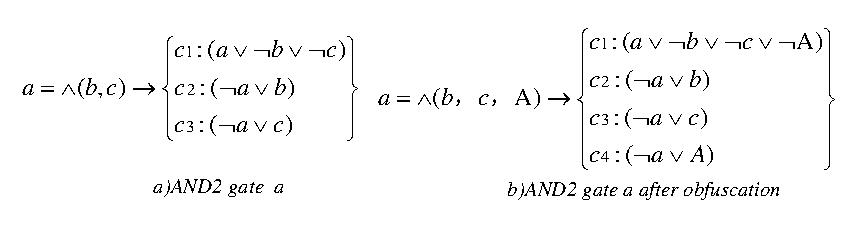
\includegraphics[width=9.2cm]{AND2.eps}}
%\caption{将AND2混淆为AND3.}\centering
%%\caption{Obfuscating AND2 into AND3.}\centering
%\label{4:fig_AND2}
%\end{figure}

\subsubsection{$OBFUSCATOR$算法}

%The proposed OBUFSCATOR algorithm obfuscates CNF formula $F_C$ with SSH rules and CSA strategies,
%so as to prevent structure of $F_C$ and its accurate solution from being known by adversary.
%
%To achieve these goals, OBFUSCATOR detect gates in CNF formula,
%then transform them into gates with different CNF signature.
%Detailed implementation of OBFUSCATOR is in Algorithm \ref{4:algo_obs}, which use $mark$ $($line \ref{4:mark}$)$ to detect key clauses and output variables  in CNF formula,
%and use $generate\_new\_clause$ $($line \ref{4:gennewclause}$)$ to generate new clause.
%As all circuits can be represented by a combination of AND2 and INV,
%and the $mark$ algorithm for INV is trivial,
%so we only present the implementation of $mark$ for AND2 in Algorithm \ref{4:algo_mark}.
%Similarly, we also present only the implementation of $\mathbf{generate\_new\_clause}$ for AND2 in Algorithm \ref{4:algo_mark}.
%These two algorithms can transform a CNF signature of AND2 to that of AND3.

$OBUFSCATOR$算法遵循上述SSH规则,
并选取具有簇形解的Husk公式$F_H$,
混淆CNF公式$F_C$,
从而防止$F_C$携带的电路结构和它的真实解被潜在的攻击者获取。

为了达到上述目标,
$OBFUSCATOR$ 首先会在CNF公式中的特征子句里随机加入新的文字,
并使用Husk公式$F_H$中的文字生成新的子句,
以改变原有公式的标记。
%OBFUSCATOR的详细实现在算法\ref{4:algo_obs}中,其中使用$mark$(第$\ref{4:mark}$行)来检测CNF公式中的关键子句和输出变量,
%并使用$generate\_new\_clause$(第$\ref{4:gennewclause}$行)产生新的子句。
%由于AND2是最常见的门,
%我们在仅仅给出AND2门的$\mathbf{mark}$算法,
%同样,我们也仅仅给出AND2的$\mathbf{generate\_new\_clause}$ 算法,
%这两个算法组合起来可以将AND2的标记转换为AND3的标记.具体的实现在算法\ref{4:algo_mark}中。

%\begin{algorithm*}[b]
%%\SetAlgoLined
%\SetAlgoNoLine
%\KwData{NULL}
%\KwResult{Husks CNF $F_H$ and Husks result $R_H$}
%\Begin{
%Generating prime numbers $p_A$ and $p_B$  \; \label{4:primenumber}
%$\Phi= M(I_1 \neq 1, I_2\neq 1, O=p_A*p_B)$ \;\label{4:multiplePrime}
%$F_H=Tseitin(\Phi)$ \;\label{4:TseitinPHI}
%$R_H=p_A\mid p_B$ \;
%}
%\caption{GENERATOR}
%\label{4:algo2_gen}
%\end{algorithm*}

%\begin{algorithm}[t]
%\SetAlgoNoLine
%\KwData{The original CNF $F_C$, Husks CNF $F_H$, Husks result $R_H$}
%\KwResult{The obfuscated CNF $F_O$, variable mapping $M$}
%\Begin{
%$mark(F_C)$\;\label{4:mark}
%\ForEach{$c\in F_C$}{
%\If{$c \in$  Key Clause Set } {\label{4:keyclause}
%    lit =get literal $ \in R_H$\;
%    $c=c \cup \neg lit$\;\label{4:rule1}
%    $nc=generate\_new\_clause(c,lit)$\;\label{4:gennewclause}
%    $F_C=F_C \cup nc$\;\label{4:blendclause1}
% }
%}
%\ForEach{$ c \in F_C $} {
%$averagelen=\frac{\sigma _{c'\in F_C}|c'|}{|F_C|}$ \;
%\While{$|c| < averagelen$}{
%$lit=$get literal $\in R_H$ \;
%\While{$\neg lit \in c$} {
%lit=get literal $ \in R_H $ \;
%}
%$c=c \cup \neg lit$\;\label{4:rule1-2}
%}
%$M$ =remap all variable in $F_C\cup F_H$ \;\label{4:MV}
%$F_O$ =reorder all clause in $F_C\cup F_H$ \; \label{4:blendclause2}
%}
%}
%\caption{OBFUSCATOR}
%\label{4:algo_obs}
%\end{algorithm}
%
%\begin{algorithm}[t]
%\SetAlgoNoLine
%$\mathbf{mark}$\;
%\KwData{CNF formula $S$}
%\KwResult{marked $S$ }
%\Begin{
%\ForEach{$(C \in S) ~\&~ (|C|\equiv 3)$}{
%\ForEach{$l \in C$ }{
%\ForEach{$(C_1 \in S) ~\&~ (\neg l\in C_1)~ \&~ (|C_1|\equiv 2)$ }{
%\ForEach{$l_1 \in C_1$ }{
%\uIf{$(\neg l_1 \in C)~\&~(l_1\ne l)$} {
%$match++$ \;
%}
%}
%}
%}
%}
%\If{$match\equiv 2$} {
%mark $l$ as output literal \;
%mark $C$ as Key Clause\;
%}
%}
%$\mathbf{generate\_new\_clause}$\;
%\KwData{key clause $C$ in AND2, Husk literal $lit$}
%\KwResult{new clause $C_1$}
%\Begin{
%$olit$=Getting output literal from $C$ \;
%$C_1= lit \cup \neg olit$ \;\label{4:rule2}
%}
%\caption{$\mathbf{mark}$ and $\mathbf{generate\_new\_clause}$}
%\label{4:algo_mark}
%\end{algorithm}

%SSH and CSA based obfuscation procedure implemented in Algorithm \ref{4:algo_obs} and \ref{4:algo_mark} is described below.
%% \textbf{SSO obfuscation with SSH rule and CSA strategy}
%\begin{Procedure}[${Obf_{SSH\_CSA}}$]\label{4:obsprocedure}~
%\begin{enumerate}
%\item Input:
%Formula $F_C$, Husks formula $F_H$, solution $R_H$.
%\item Output:
%Formula $F_O$.
%\end{enumerate}
%According to Algorithm \ref{4:algo_obs},
%$F_C$ consists of \textbf{key clause}(line \ref{4:keyclause}) and \textbf{non-key clause},
%corresponding clause sets denoted as \textbf{$F_{Ck}$} and \textbf{$F_{Cn}$}.
%
%% $~~~~R_H$ is one sultion of $F_H$.
%\textbf{Step 1}:
%For key clause $c\in F_{Ck}$,
%take one literal lit from $R_H$,
%and insert $\neg lit$ into $c$ (at line \ref{4:rule1}, \ref{4:rule1-2} in Algorithm \ref{4:algo_obs})  according to  SSH rule 1.
%% if variable is $T$ in $R_H$, insert its negative literal;
%% if variable is $F$ in $R_H$, insert its positive literal.
%The resulting clause set is denoted as $S_3$ .
%
%\textbf{Step 2}:
%Generating new clauses  (line \ref{4:gennewclause} in Algorithm \ref{4:algo_obs}) with literal lit from $R_H$ and output variable of $c$ in $F_C$ according to SSH rule 2 (line \ref{4:rule2} in Algorithm \ref{4:algo_mark}).
%% %generating new clauses with literals from $R_H$ and variables in $F_C$ according to the SSH rule 2:
%% if variable is $T$ in $R_H$, insert positive literal into clause;
%% if variable is $F$ in $R_H$, insert negative literal into clause;
%% %Literal of output variable is extracted directly from the key clause and inverted.
%New clauses set generated in this way is denoted as $S_4$.
%
%\textbf{Step 3}:
%Combining and randomly reordering $S_3$, $S_4$, $F_H$, and $F_{Cn}$, to produce $F_O$ (line \ref{4:rule1}, \ref{4:rule1-2}, \ref{4:blendclause1} \ref{4:blendclause2} in Algorithm \ref{4:algo_obs}).
%
%\textit{\textbf{end Procedure}}.
%\end{Procedure}
%
%算法\ref{4:algo_obs}和\ref{4:algo_mark}中实现的

基于SSH规则的SPE混淆过程逻辑步骤描述如下。

\textit{\textbf{Procedure \ref{4:obsprocedure}}}.
% \textbf{SSO obfuscation with SSH rule and CSA strategy}
%\begin{procedure}[${Obf_{SSH\_CSA}}$]\label{4:obsprocedure}~
\begin{enumerate}
\item[]\label{4:obsprocedure} 输入:公式$F_C$(其中包含了\textbf{关键子句集合$F_{Ck}$}
和\textbf{非关键子句集合$F_{Cn}$}),Husks 公式$F_H$以及其解$R_H$。
\item[] 输出:混淆结果$F_O$。
\end{enumerate}

\textbf{步骤1}:
对关键子句$c\in F_{Ck}$,
从$R_H$中取出文字$lit$。
根据SSH规则1,
将$\neg lit$加入到$c$。
按照该规则生成的子句集合记为$S_3$ .

\textbf{步骤2}:
根据SSH规则2,
使用$R_H$中文字$lit$和$c$中的输出变量,产生新的子句。
新产生的子句集合记为$S_4$.

\textbf{步骤3}:
将$S_3$,$S_4$,$F_H$和$F_{Cn}$混合产生$F_O$。

\textit{\textbf{end Procedure}}.
%\end{procedure}
\subsection{解恢复和验证算法}\label{4:mappping}
%After SAT Solving finished in public Cloud, $S_O$,
%the solution of $F_O$, will be returned to the private Cloud.
%In accordance with OBFUSCATOR,
%MAPPER and VERIFIER are used to filter solution of $F_C$ out from  $S_O$.
%MAPPER and VERIFIER are implemented in Algorithm \ref{4:algo_map}.
%
%According to Theorem \ref{4:SSOtheorem},
%If result is UNSAT, then the original CNF formula is UNSAT (line \ref{4:sUNSAT}).
%If result is SAT, MAPPER (line \ref{4:var}-\ref{4:mapper}) projects solution into variables of $F_C$ and $F_H$,
%to get $S_C$ and $S_H$, which are the candidate solution of $F_C$ and $F_H$ respectively.
%VERIFIER (line \ref{4:verifer1}-\ref{4:verifer2}) checks if $S_H$ is equal to $R_H$,
%if yes, $S_C$ is real solution of  $F_C$.
%Otherwise, $S_C$ may be false solution,
%hence, it is necessary to ask for a new solution from SAT Solver(at line \ref{4:Warning}).
%
%The solution projection is done according to the variable mapping table $M$,
%generated by OBFUSCATOR(at Line \ref{4:MV} in Algorithm \ref{4:algo_obs}).
%$M[var].variable$ (at Line \ref{4:var}) represents the original variables name of var,
%and $M[var].formula$ (at Line \ref{4:formula}) may be $F_C$ or $F_H$, which the var belongs to.

在公共云上的求解器完成求解,
并将$F_O$的解$S_O$返回给私有云。
和混淆器相对应,
在私有云中使用算法\ref{3:algo_map}中的$MAPPER$和$VERIFIER$将$F_C$的解从$S_O$中过滤出来。
解的恢复和验证算法和第\ref{chap:3}章相同。
%MAPPER和VERIFIER的实现在算法\ref{4:algo_map}中.
%
%根据定理\ref{4:SPEtheorem},
%如果结果是UNSAT, 那么原始的CNF公式也是(第\ref{4:sUNSAT}行).
%如果结果是SAT, MAPPER(\ref{4:var}-\ref{4:mapper} 行)将解投影到$F_C$和$F_H$的变量上,
%已获得$S_C$ 和$S_H$,分别作为$F_C$和$F_H$的候选解。
%VERIFIER (\ref{4:verifer1}-\ref{4:verifer2} 行)检测$S_H$是否等于$R_H$,
%如果等于, $S_C$就是$F_C$的真实解.
%否则, $S_C$ 可能是假解,
%此时,需要从SAT求解器获得一个新的解(第\ref{4:Warning}行).
%
%解的投影过程依赖于变量映射表$M$,它由OBFUSCATOR(算法\ref{4:algo_obs}的\ref{4:MV} 行)创建.
%$M[var].variable$ (第\ref{4:var}行)表示了var的原始变量名,
%$M[var].formula$ (第\ref{4:formula}行)表示var 所属于的公式,可以是$F_C$ 或 $F_H$。

\section{理论分析和证明}
%\section{正确性,有效性和算法复杂性}
\subsection{正确性证明}\label{4:correctness}

%According to Theorems \ref{4:SSEtheorem} and \ref{4:SSOtheorem}, under SSH rules,
%original CNF formula can be blended with Husks formula seamless, without narrowing down the solution space.
%In this section, we prove these theorems.
%First of all, let's introduce some lemmas.
根据定理\ref{4:SSPEtheorem},在SSH规则下,
原始的CNF公式可以和Husks公式无缝混合, 并会保持解空间的投影等价。
本节证明这些定理。
在证明之前,首先给出以下的引理。

\begin{lemma}[Cubic Husks Equation(CHE)]\label{4:CHE}

对簇形Husk公式 ${F_H}$,
记$|V_{F_H}|= n$。
其公共赋值变量集合$R_H=\{c_i|1\leqslant i\leqslant n_c\}$,
其中$n_c$为簇形解中公共赋值变量的个数。
它的全部$m$个解记为$\{S_{H_l}|1\leqslant l\leqslant m $且 $m \geqslant 2\}$。
其中每个解记为
$S_{H_l}=\{c_i=B_i, y_{l_i}=B_{l_i}|B_i,B_{l_i} \in \{T,F\}, 1\leqslant i\leqslant n_c \lessdot {l_i}\leqslant n\}$。


根据公共赋值变量集合$R_H$,令$F_{_RH}=
(\bigwedge_{1\leqslant i\leqslant n_c}^{B_i\equiv T} c_i)\wedge
(\bigwedge_{1\leqslant j\leqslant n_c}^{B_j\equiv F}\neg c_j)$。
%(\bigwedge_{n_c\lessdot l_i\leqslant n}^{B_{l_i}\equiv T} y_i)\wedge
%(\bigwedge_{n_c\lessdot l_j\leqslant n}^{B_{l_j}\equiv F}\neg y_j)$

则对簇形Husk公式的任一解$S_{H_l}$,令$F_{slH}=F_{_RH}\wedge
(\bigwedge_{n_c\lessdot l_i\leqslant n}^{B_{l_i}\equiv T} y_{l_i})\wedge
(\bigwedge_{n_c\lessdot l_j\leqslant n}^{B_{l_j}\equiv F}\neg y_{l_j})$。

并且令$F_{_SH}=\bigvee_{1\leqslant l\leqslant m}F_{slH}$。

\textbf{则有}  $F_{_SH} \equiv F_H $。
\end{lemma}

\begin{proof}

1) 由于 $F_{_SH}$可满足,则必然存在可满足公式:
% $F_{slH}\equiv T$, for
\begin{equation}
F_{slH}=F_{_RH}\wedge
(\bigwedge_{n_c\lessdot l_i\leqslant n}^{B_{l_i}\equiv T} y_{l_i})\wedge
(\bigwedge_{n_c\lessdot l_j\leqslant n}^{B_{l_j}\equiv F}\neg y_{l_j})
%(\bigwedge_{1\leqslant i\leqslant n_c}^{C_i\equiv T} y_i)\wedge
%(\bigwedge_{1\leqslant j\leqslant n_c}^{C_j\equiv F}\neg y_j)\wedge
%(\bigwedge_{n_c\lessdot l_i\leqslant n}^{B_{l_i}\equiv T} y_i)\wedge
%(\bigwedge_{n_c\lessdot l_j\leqslant n}^{B_{l_j}\equiv F}\neg y_j)
\end{equation}
则有:
\begin{multline}
%S_{H_l}=\{y_{i}=T,y_{j}=F|B_{l_i}\equiv T, B_{l_j}\equiv F, 1\leqslant i, j\leqslant n \}
S_{H_l}=\{c_{i}=T,c_{j}=F,y_{l_i}=T,y_{l_j}=F|
\\
B_i\equiv T, B_j\equiv F,
B_{l_i}\equiv T, B_{l_j}\equiv F, 
1\leqslant i,j\leqslant n_c,
n_c\lessdot l_i,l_j\leqslant n,
\}
\end{multline}
令$B_i,B_{l_i}$和$B_j,B_{l_j}$分别替换$c_{i}=T$,$y_{l_i}=T$中的$T$和$c_{j}=F$、$y_{l_j}=F$中的$F$, 则有:
\begin{multline}\label{4:SHL}
S_{H_l}=\{(c_i=B_i,c_j=B_j,y_{l_i}=B_{l_i},y_{l_j}=B_{l_j})|
\\
B_i\equiv T, B_j\equiv F, 1\leqslant i, j\leqslant n_c,
B_{l_i}\equiv T, B_{l_j}\equiv F, n_c\leqslant l_i, l_j\leqslant n
\}
\end{multline}

下标$i$和$j$取值范围相同,统一用$i$表示。
下标$l_i$和$l_j$取值范围相同,统一用$l_i$表示。
则式\ref{4:SHL}可以简化表示为:
\begin{equation}
S_{H_l}=\{c_i=B_i, y_{l_i}=B_{l_i}|B_i,B_{l_j} \in \{T,F\}, 1\leqslant i\leqslant n_c \lessdot l_i\leqslant n\}
\end{equation}

因为$S_{H_l}$是$F_H$的一个解,则有$F_H(S_H/V_{F_H})\equiv T$。 则有:
\begin{equation}\label{4:left}
 F_{_SH} \vdash F_H
\end{equation}

2) 由于 $F_H$可满足,
必然存在$F_H$的解,如式(\ref{4:solution_hl})所示, 可以使$F_H(S_{H_1}/V_{F_H})$ 为真。
\begin{equation}\label{4:solution_hl}
S_{H_1}=\{c_i=B_i, y_{l_i}=B_{l_i}|B_i,B_{l_i} \in \{T,F\}, 1\leqslant i\leqslant n_c \lessdot l_j\leqslant n\}
%S_{H_1}=\{y_k=B_{1_k}|B_{1_k} \in \{T,F\}, 1\leqslant k\leqslant n\}.
\end{equation}
根据式(\ref{4:solution_hl}) 构造 $F_{s1H}$ ,则有:
%式(\ref{4:SH})
\begin{equation}\label{4:s1H}
F_{s1H}=
(\bigwedge_{1\leqslant i\leqslant n_c}^{B_i\equiv T} c_i)\wedge
(\bigwedge_{1\leqslant j\leqslant n_c}^{B_j\equiv F}\neg c_j)\wedge
(\bigwedge_{n_c\lessdot l_i\leqslant n}^{B_{l_i}\equiv T} y_i)\wedge
(\bigwedge_{n_c\lessdot l_j\leqslant n}^{B_{l_j}\equiv F}\neg y_j)
 \equiv T
%F_{s1H}=
%(\bigwedge_{1\leqslant i\leqslant n_1}^{B_{1_i}\equiv T}y_{i})\wedge
%(\bigwedge_{1\leqslant j\leqslant n_1}^{B_{1_j}\equiv F}\neg y_{j})\wedge
%(\bigwedge_{1\leqslant i\leqslant n_2}^{C_{i}\equiv T}y_{i})\wedge
%(\bigwedge_{1\leqslant j\leqslant n_2}^{C_{j}\equiv F}\neg y_{j})
\end{equation}
\begin{equation}\label{4:SH}
F_{_SH} =F_ {s1H} \vee (\bigvee_{2\leqslant l\leqslant m}F_{slH}). \\
\end{equation}
因为$F_{s1H} \equiv T$, 根据式(\ref{4:s1H})和(\ref{4:SH}), 则有:
\begin{equation}
F_{_SH} \equiv T
\end{equation}
\begin{equation}\label{4:right}
F_H \vdash F_{_SH}
\end{equation}
根据公式(\ref{4:left})和(\ref{4:right}), 则有:
\begin{equation}
 F_{_SH} \equiv F_H
\end{equation}
%\textit{end proof.}

证明完成。
\end{proof}

%
%\begin{lemma}[Husks Equation(HE)]\label{4:HE}
%
%对Husks公式 ${F_H}$且$|V_{F_H}|= n$,
%它的全部$m$解$\{S_{H_l}|1\leqslant l\leqslant m\}$,
%且解$S_{H_l}=\{y_k=B_{l_k}|B_{l_k} \in \{T,F\}, 1\leqslant k\leqslant n\}$.
%
%对每个$S_{H_l}$, 令$F_{slH}=
%(\bigwedge_{1\leqslant i\leqslant n}^{B_{l_i}\equiv T}y_{i})\wedge
%(\bigwedge_{1\leqslant j\leqslant n}^{B_{l_j}\equiv F}\neg y_{j})$,
%
%并且令$F_{_SH}=\bigvee_{1\leqslant l\leqslant m}F_{slH}$,
%
%\textbf{则有}  $F_{_SH} \equiv F_H $.
%\end{lemma}
%
%\begin{proof}
%
%1) 由于 $F_{_SH} \equiv T$ 则必然存在
%% $F_{slH}\equiv T$, for
%\begin{equation}
%F_{slH}=
%(\bigwedge_{1\leqslant i\leqslant n}^{B_{l_i}\equiv T}y_{i})\wedge
%(\bigwedge_{1\leqslant j\leqslant n}^{B_{l_j}\equiv F}\neg y_{j}) \equiv T
%\end{equation}
%则有:
%\begin{equation}
%S_{H_l}=\{y_{i}=T,y_{j}=F|B_{l_i}\equiv T, B_{l_j}\equiv F, 1\leqslant i, j\leqslant n \}
%\end{equation}
%令$B_i$, $B_j$分别替换$y_{i}=T$中的$T$和$y_{j}=F$ 中的$F$, 则有:
%\begin{equation}
%S_{H_l}=\{(y_i=B_{l_i},y_j=B_{l_j})|B_{l_i}\equiv T, B_{l_j}\equiv F, 1\leqslant i, j\leqslant n\}
%\end{equation}
%因为$S_{H_l}$是$F_H$的一个解,则有$F_H(S_H/V_{F_H})\equiv T$。 则有:
%\begin{equation}\label{4:left}
% F_{_SH} \vdash F_H
%\end{equation}
%2) 由于 $F_H\equiv T$, 必然存在$F_H$的解,如式(\ref{4:solution_hl})所示, 可以使$F_H(S_{H_1}/V_{F_H})$ 为真。
%\begin{equation}\label{4:solution_hl}
%S_{H_1}=\{y_k=B_{1_k}|B_{1_k} \in \{T,F\}, 1\leqslant k\leqslant n\}.
%\end{equation}
%根据式(\ref{4:solution_hl}) 构造 $F_{s1H}$ ,则有式(\ref{4:SH}):
%\begin{equation}\label{4:s1H}
%F_{s1H}=
%(\bigwedge_{1\leqslant i\leqslant n}^{B_{1_i}\equiv T}y_{i})\wedge
%(\bigwedge_{1\leqslant j\leqslant n}^{B_{1_j}\equiv F}\neg y_{j})
%\end{equation}
%\begin{equation}\label{4:SH}
%F_{_SH} =F_ {s1H} \vee (\bigvee_{2\leqslant l\leqslant m}F_{slH}). \\
%\end{equation}
%因为$F_{s1H} \equiv T$, 并且有式(\ref{4:s1H})和(\ref{4:SH}), 则有:
%\begin{equation}
%F_{_SH}  \equiv T
%\end{equation}
%\begin{equation}\label{4:right}
%F_H \vdash F_{_SH}
%\end{equation}
%According to Equation (\ref{4:left}) and (\ref{4:right}), 则有:
%\begin{equation}
% F_{_SH} \equiv F_H
%\end{equation}
%%\textit{end proof.}
%\end{proof}
%
%\begin{lemma}[Singular Husk Equation(SHE)]\label{4:SHE}
%
%对单一Husk公式${F_H}$且有$|V_{F_H}|= n$,
%其唯一解$S_H$=$\{(y_i=B_i,y_j=B_j)|B_i\equiv T, B_j\equiv F, 1\leqslant i, j\leqslant n \}$.
%
%令$F_{_SH}=F_H\wedge (\bigwedge_{1\leqslant i\leqslant n}^{B_i\equiv T}y_i)\wedge(\bigwedge_{1\leqslant j\leqslant n}^{B_j\equiv F}\neg y_j)$
%
%\textbf{则有} $F_H \equiv F_{_SH}$.
%\end{lemma}
%\begin{proof}~\\
%1)因为$F_H\equiv T$, $F_H$ 有唯一解$S_H$。
% \begin{equation}\label{4:S_H}
% S_H=\{(y_i=B_i,y_j=B_j)|B_i\equiv T, B_j\equiv F, 1\leqslant i, j\leqslant n \}.
%\end{equation}
%根据式\ref{4:S_H}),构造$F_{_{lS}H}$
%\begin{equation}
% F_{_{lS}H}=(\bigwedge_{1\leqslant i\leqslant n}^{B_i\equiv T}y_i)\wedge(\bigwedge_{1\leqslant j\leqslant n}^{B_j\equiv F}\neg y_j)
%\end{equation}
%则有
%\begin{equation}
% F_{_{lS}H} \equiv T
%\end{equation}
%构造$F_{_SH}$
%\begin{equation}
% F_{_SH}=F_H\wedge F_{_{lS}H}
%\end{equation}
%则有
%\begin{equation}
% F_{_SH} \equiv T
%\end{equation}
%\begin{equation}
% F_H \vdash F_{_SH}
%\end{equation}\\
%2)因为 $F_{_SH}\equiv T$
%\begin{equation}
%F_{_SH}=(\bigwedge_{1\leqslant i\leqslant n }^{B_i\equiv T}y_i)\wedge(\bigwedge_{1\leqslant j\leqslant n}^{B_j\equiv F}\neg y_j)
%\end{equation}
%则有$F_{_SH}$的唯一解$S_H$
%\begin{equation}
%S_H=\{(y_i=T,y_j=F)|B_i\equiv T, B_j\equiv F, 1\leqslant i, j\leqslant n \}
%\end{equation}
%令 $B_i$替换$T$, $B_j$替换$F$,则有
% \begin{equation}
%S_H=\{(y_i=B_i,y_j=B_j)|B_i\equiv T, B_j\equiv F, 1\leqslant i, j\leqslant n \}
% \end{equation}
%因为$S_H$是$F_H$的解, 则有
%\begin{equation}
%F_H(S_H/V_{F_H})\equiv T
%\end{equation}
% 因此有
% \begin{equation}
%  F_H \vdash F_{_SH}
% \end{equation}
% \\
%因为 1) and 2):
%\begin{equation}
% F_H \equiv F_{_SH}.
%\end{equation}
%\end{proof}
%
%
%根据Lemma \ref{4:HE}和\ref{4:SHE},一个单一Husk公式等价于解文字的合取;
%一个Husks公式等价于解子句的析取,其中每个解子句是该解中所有文字的合取。
%
%\begin{lemma}[OR Hold Obfuscation]\label{4:ORrelation-Holding-Obfuscation}
%对公式$F_C$ 和$F_{_RH}\vee F_{_SH}$,及$F_{_RH} \vee F_{_SH}$的一个赋值$R_H$ 有,
%
%$Obf(F_C,F_{_RH}\vee F_{_SH},R_H)\equiv Obf(F_C,F_{_RH},R_H) \vee Obf(F_C,F_{_SH},R_H)$
%\end{lemma}
%\begin{proof}
%假设:
%\begin{enumerate}
% \item[-]$F_C$=$F_{Ck} \wedge F_{Cn}$,  $F_{Ck}$= $\bigwedge_{1}^{m}(a_i\vee X_i$).
% \item[-]$F_H$=$F_{_RH}\vee F_{_SH}$
% \item[-]$R_H$=$\{y_j=B_j| B_j \in \{T,F\}, 1\leqslant j\leqslant n\}$.
% \item[-]令 $F_O=Obf(F_C,F_H,R_H)$
% \end{enumerate}
%
%根据\textbf{Procedure}\ref{4:obsprocedure}, 按下列3个\textbf{步骤}构造$F_O$.
%\begin{enumerate}
%\item  $(y_j\equiv B_j)\in$ $R_H$, $(a_i\vee X_i) \in F_{Ck}$和规则1:
%\begin{itemize}
% \item[] 如果$B_j\equiv T$, 则子句$C_{ij}=(a_i\vee X_i)\wedge \neg y_j$.
% \item[] 如果$B_j\equiv F$, 则子句$C_{ij}=(a_i\vee X_i)\wedge y_j$.
%\end{itemize}
%令$S_3=\bigwedge_{1\leqslant i\leqslant m}^{1\leqslant j\leqslant n} C_{ij}$
%\item
%$(y_j\equiv  B_j)\in $ $R_H$, $(a_i\vee X_i) \in F_{Ck}$以及规则2:
%\begin{itemize}
% \item[] 如果$B_j\equiv T$, 则子句$D_{ij}=\neg a_i\wedge y_j$.
% \item[] 如果$B_j\equiv F$, 则子句$D_{ij}=\neg a_i\wedge \neg y_j$.
%\end{itemize}
%令$S_4=\bigwedge_{1\leqslant i\leqslant m}^{1\leqslant j\leqslant n} D_{ij}$.
%\item\label{4:ORFO}
%令$F_{_dC} =S_3\wedge S_4 \wedge F_{Cn}$, then $F_O=F_H \wedge F_{_dC}$.
%\end{enumerate}
%根据步骤\ref{4:ORFO}):
%\begin{equation}\label{4:FOOBF}
%\begin{array}{ccc}
%F_O  =  F_H \wedge F_{_dC}                                   &F_H=F_{_RH}\vee F_{_SH}&\models\\
%F_O  =  (F_{_RH}\vee F_{_SH})\wedge F_{_dC}                  &                       &\models\\
%F_O  =  (F_{_RH} \wedge F_{_dC})\vee(F_{_SH}\wedge F_{_dC})  &                       &
%\end{array}
%\end{equation}
%根据\textbf{Procedure}\ref{4:obsprocedure}, $F_{_dC}$仅和$F_C$以及$R_H$ 相关, 则\\
%% \begin{equation}
%%  Obf(F_C,F_H,R_H) \equiv F_H \wedge F_{_dC}
%% \end{equation}
%\begin{equation}\label{4:SHOBF}
%F_{_SH} \wedge F_{_dC} \equiv Obf(F_C,F_{_SH},R_H)
%\end{equation}
%\begin{equation}\label{4:RHOBF}
%F_{_RH} \wedge F_{_dC} \equiv Obf(F_C,F_{_RH},R_H)
%\end{equation}
%根据式(\ref{4:FOOBF}), (\ref{4:SHOBF}), (\ref{4:RHOBF}), 有:
% \begin{equation}
%F_O \equiv Obf(F_C,F_{_RH} ,R_H)
%\vee Obf(F_C,F_{_SH} ,R_H)
% \end{equation}
%
%%\textit{end proof.}
%\end{proof}
%
%% \begin{lemma}[AND Hold Obfuscation]\label{4:ANDrelation-Holding-Obfuscation}
%\begin{lemma}[AND Hold Obfuscation]\label{4:ANDrelation-Holding-Obfuscation}
%公式$F_C$ 和$F_{_RH}\wedge F_{_SH}$,
%并且$R_H$是$F_{_RH} \wedge F_{_SH}$的一个赋值, 则有
%
%$Obf(F_C,F_{_RH} \wedge F_{_SH},R_H) $ \\
%$\equiv Obf(F_C,F_{_RH},R_H) \wedge Obf(F_C,F_{_SH} ,R_H)$
%\end{lemma}
%\begin{proof}
%%\textsl{略.}
%%同Lemma \ref{4:ORrelation-Holding-Obfuscation}.
% \textbf{Assume}
% \begin{enumerate}
% \item[-] Clause $A=a\vee X$,and clause $B=b$, while $b\notin X$,arbitary formula $F_{Cn},F_{_SH}$
% \item[-] Let $F_{Ck} =A, F_C=F_{Ck} \wedge F_{Cn}$, \\
%           $F_{_RH}=B, F_H=F_{_RH}\wedge F_{_SH}$, while $R_H=\{b\equiv T\}$;
% \item[-] Let $F_O=Obf(F_C,F_H,R_H)$
% \end{enumerate}
% % then $F_O=Obf(F_C,F_{_RH},R_H)\wedge Obf(F_C,F_{_SH},R_H)$.
% 根据\textbf{Procedure} \ref{4:obsprocedure}, 按下列3个步骤构造$F_O$。
% \begin{enumerate}
% \item 根据$R_H$和规则1,
% we have clause $C=A\vee \neg b$, and $S_3=C$
% \item
% With $R_H$ and Rule 2,
% with literal $a\in A$,
% we have clause $D=\neg a\vee b$;
% and $S_4=D$;
% \item
% Let  $F_{_dC} =S_3\wedge S_4 \wedge F_{Cn}$.\\
% then $F_O=F_H \wedge F_{_dC}$.
% \end{enumerate}
% \begin{equation}\label{4:ANDequation}
% \begin{array}{ccc}
% F_O  =  F_H \wedge F_{_dC}                                     & F_H=F_{_RH}\wedge F_{_SH}&\models\\
% F_O  =  (F_{_RH}\wedge F_{_SH})\wedge F_{_dC}                   &                        &\models\\
% F_O  =  (F_{_RH} \wedge F_{_dC})\wedge (F_{_SH} \wedge F_{_dC})  &                        &\models\\
% \end{array}
% \end{equation}
% 根据\textbf{Procedure} \ref{4:obsprocedure}, $F_{_dC}$仅仅和$F_C$、$R_H$ 相关, 则
%\begin{equation}\label{4:FSHequation}
% F_{_SH} \wedge F_{_dC} \equiv Obf(F_C,F_{_SH},R_H)
%\end{equation}
%\begin{equation}\label{4:FRHequation}
% F_{_RH} \wedge F_{_dC} \equiv Obf(F_C,F_{_RH},R_H)
%\end{equation}
%根据式\ref{4:ANDequation})、\ref{4:FSHequation})和\ref{4:FRHequation}),则有
%\begin{equation}
% F_O  = Obf(F_C,F_{_RH},R_H)\wedge Obf(F_C,F_{_SH},R_H)
%\end{equation}
%\
%textit{end proof.}
%\end{proof}
%
%根据Lemma\ref{4:ORrelation-Holding-Obfuscation} 和\ref{4:ANDrelation-Holding-Obfuscation},
%对Husks公式$F_H$,  AND和OR 关系在混淆后依然保持。
%
%\begin{lemma}[Unique Positive literal SSE Obfuscation]\label{4:UPSSE-lemma}
%% \textbf{(Unique Positive literal SSE Obfuscation)}
%任意公式$F_C$, 有
%
%\textbf{$Obf(F_C,B=b,{b\equiv T})\equiv F_C\wedge b$}
%\end{lemma}
%\begin{proof}
%%\textbf{Unique Positive literal SSE Obfuscation (UPSSE)}:\label{4:UPSSE-lemma}
%假设
%\begin{enumerate}
% \item[-]$F_C$=$F_{Ck} \wedge F_{Cn}$, $F_{Ck}=A$, $A=a\vee X$.
% \item[-]$F_H$=$B$, $B=b$~while $b\notin X$, $R_H$=$\{b\equiv T\}$.
% \item[-]Let $F_O=Obf(F_C,F_H,R_H)$
% \end{enumerate}
%
%根据\textbf{Procedure} \ref{4:obsprocedure}, 按下列3个步骤构造$F_O$。
%\begin{enumerate}
%\item $(b\equiv T) \in $ $R_H$以及规则1,
%有子句$C=A\vee \neg b$, 并且 $S_3=C$.
%\item
%($b\equiv T) \in $ $R_H$, literal $a\in A$和规则2,
%有子句$D=\neg a\vee b$,
%令$S_4=D$.
%\item \label{4:UPSSEFO}
%令$F_O=F_H \wedge S_3\wedge S_4 \wedge F_{Cn}$.
%\end{enumerate}
%根据步骤\ref{4:UPSSEFO}):
%\begin{equation}
%\begin{array}{ccc}
%F_O  =  F_H \wedge S_3\wedge S_4\wedge F_{Cn}           &S_3=C~ S_4=D              &\models\\
%F_O  =  F_H\wedge C\wedge D\wedge F_{Cn}                &F_H=B~ B=b                &\models\\
%F_O  =  b\wedge C\wedge D\wedge F_{Cn}                  &C=A\vee \neg b~           &\models\\
%F_O  =  b\wedge (A\vee \neg b) \wedge D\wedge F_{Cn}    &                          &\models\\
%F_O  =  b\wedge A \wedge D\wedge F_{Cn}                 & D=\neg a\vee b~          &\models\\
%F_O  =  b\wedge A \wedge (\neg a\vee b)\wedge F_{Cn}    &                          &\models\\
%F_O  =  b\wedge A \wedge F_{Cn}                         &F_{Ck} =A                 &\models\\
%F_O  =  b\wedge F_{Ck}\wedge F_{Cn}                     & F_C=F_{Ck} \wedge F_{Cn} &\models\\
%F_O  =  F_C \wedge b                                    &   &
%\end{array}
%\end{equation}
%%\textit{end proof.}
%\end{proof}
%
%\begin{lemma}[Unique Negative literal SSE Obfuscation]\label{4:UNSSE-lemma}
%任意公式$F_C$, 有
%
% \textbf{$Obf(F_C,B=\neg b,{b=F})=F_C\wedge \neg b$}
%% % Lemma \ref{4:UNSSE-lemma} can be expressed as following:
%\end{lemma}
%
% \begin{proof}
%
% \begin{enumerate}
% \item Clause $A=a\vee X$, arbitary formula $F_{Cn}$ and clause $B=\neg b$, while $b\notin X$;
% \item Let $F_{Ck} =A, F_C=F_{Ck} \wedge F_{Cn}$, $F_H=B$, while $R_H=\{b\equiv F\}$;
% \item Let $F_O=Obf(F_C,F_H,R_H)$
% \end{enumerate}
%  ~~~~then $F_O=F_C\wedge F_H$.
%
% According to \textbf{Procedure} \ref{4:obsprocedure}, Construct $F_O$ as following 3 steps.
% \begin{enumerate}
% \item[Step1]
% With $R_H$ and Rule 1,
% we have clause $C=A\vee b$;and $S_3=C$
% \item[Step2]
% With $R_H$ and Rule 2,
% with literal $a\in A$,
% we have clause $D=\neg a\vee \neg b$;
% and $S_4=D$;
% \item[Step3] let $F_O=F_H \wedge S_3\wedge S_4 \wedge F_{Cn} $.
% \end{enumerate}
% \begin{equation}
% \begin{array}{ccc}
% F_O  =  F_H \wedge S_3\wedge S_4\wedge F_{Cn}                      &F_H=B      &\models\\
% F_O  =  B \wedge S_3\wedge S_4\wedge F_{Cn}                        &S_3=C      &\models\\
% F_O  =  B \wedge C\wedge S_4\wedge F_{Cn}                          &S_4=D      &\models\\
% F_O  =  B\wedge C\wedge D\wedge F_{Cn}                             &B=\neg b                    &\models\\
% F_O  =  \neg b\wedge C\wedge D\wedge F_{Cn}                        &C=A\vee b               &\models\\
% F_O  =  \neg b\wedge (A\vee  b) \wedge D\wedge F_{Cn}              &                            &\models\\
% F_O  =  \neg b\wedge A \wedge D\wedge F_{Cn}                       &D=\neg a\vee \neg b     &\models\\
% F_O  =  \neg b\wedge A \wedge (\neg a\vee \neg b)\wedge F_{Cn}     &                            &\models\\
% F_O  =  \neg b\wedge A \wedge F_{Cn}                               &F_{Ck}=A                    &\models\\
% F_O  =  \neg b\wedge F_{Ck}\wedge F_{Cn}                        & F_C=F_{Ck} \wedge F_{Cn}   &\models\\
% F_O  =  F_C\wedge \neg b                                           &   &
% \end{array}
% \end{equation}
%
% \textit{end proof.}
% \end{proof}
%
%根据Lemma \ref{4:UPSSE-lemma}和\ref{4:UNSSE-lemma},
%单文字混淆后解空间保持等价。
%%%%%%%%%%%%%%%%%%%%%%%%%%%%%%%%%%%%%%%%%%%%%%%%%%%%%%%%%%%%%%%%%%%%%%%%%%%%%%%%%%%%%%%%%%%%%%%%%%%%%%%%%%%%%%%%%%%%%%%
%
%%Then let's discuss SSE Obfuscation based on singular Husk formula,
%%and SSO Obfuscation based on Husks formula.
%%
%%\textbf{Theorem \ref{4:SSEtheorem} Solution Space Equated (SSE) Obfuscation}
%%
%%For arbitrary CNF formula $F_C$, and Singular Husk formula $F_{_SH}$, if
%%\begin{enumerate}
%% \item[-] $V_{F_C}$ $\cap$ $V_{F_H}$ = $\phi$, $R_H$ is unique solutions of $F_H$.
%% \item[-] $F_O=Obf(F_C,F_H,R_H)$.
%%\end{enumerate}
%%~~~then  $F_C\wedge F_H \equiv F_O$.
%%\begin{proof}
%%
%%Assume $R_H$=$\{y_k=B_k| B_k \in \{T,F\}, 1\leqslant k\leqslant n\}$.
%%
%%According to \textbf{Procedure} \ref{4:obsprocedure}, constuct $F_O$ as following \textbf{steps}:
%%\begin{enumerate}
%%\item \label{4:Fop}
%%Let $F_{Op}=F_C$.  \\
%%% for all $B_i\equiv T$, let
%%for $y_i \in \{y_i|(y_i=B_{i})\in R_H \parallel B_i\equiv T)\}$, let
%%\begin{itemize}
%% \item[] $F_{Op}$=$Obf(F_{Op},B=y_i,{y_i\equiv B_i})$.
%%\end{itemize}
%%\item  \label{4:Fonp}
%%Let $F_{On}=F_{Op}$. \\
%%% for all $B_j\equiv F$, let
%%for $y_j \in \{y_j|(y_j=B_j)\in R_H \parallel B_j\equiv F)\}$, let
%%\begin{itemize}
%% \item[] $F_{On}$= $Obf(F_{On},B=\neg y_j,{y_j\equiv B_j})$.
%%\end{itemize}
%%\item  \label{4:SSEFOend}
%%$F_{O}=F_{On}\wedge F_H$.
%%\end{enumerate}
%%According to Lemma \ref{4:ANDrelation-Holding-Obfuscation}, \ref{4:UPSSE-lemma} and Step \ref{4:Fop}), we have:
%%\begin{equation}\label{4:SSEFOP}
%%F_{Op} \equiv F_C\wedge (\bigwedge_{1\leqslant i\leqslant n}^{B_i \equiv T}y_i)
%%\end{equation}
%%According to Lemma \ref{4:ANDrelation-Holding-Obfuscation}, \ref{4:UNSSE-lemma} and Step \ref{4:Fonp}), we have:
%%\begin{equation}\label{4:SSEFON}
%%F_{On} \equiv F_{Op}\wedge (\bigwedge_{1\leqslant j\leqslant n}^{B_j \equiv F}\neg y_j).
%%\end{equation}
%%% then
%%% \begin{equation}\label{4:SSEOPN}
%%% F_{On} \equiv F_C \wedge
%%% (\bigwedge_{1\leqslant i\leqslant n}^{B_i \equiv T}y_i)\wedge
%%% (\bigwedge_{1\leqslant j\leqslant n}^{B_j \equiv F}\neg y_j)\\
%%% \end{equation}
%%According to Step \ref{4:SSEFOend}) and Equation (\ref{4:SSEFOP}) (\ref{4:SSEFON}), we have:
%%\begin{equation}\label{4:SSEFO}
%%F_{O} \equiv F_C \wedge
%%(\bigwedge_{1\leqslant i\leqslant n}^{B_i \equiv T}y_i)\wedge
%%(\bigwedge_{1\leqslant j\leqslant n}^{B_j \equiv F}\neg y_j) \wedge F_H
%%\end{equation}
%%Since ${R_H}$ is the unique satisfied solution of $F_H$,
%%according to Lemma \ref{4:SHE}, we have:
%%\begin{equation}\label{4:SSEFH}
%%F_H \wedge (\bigwedge_{1\leqslant i\leqslant n}^{B_i \equiv T}y_i)\wedge
%%(\bigwedge_{1\leqslant j\leqslant n}^{B_j\equiv F}\neg y_j)\equiv F_H
%%\end{equation}
%%According to Equation (\ref{4:SSEFO}), (\ref{4:SSEFH}), we have:
%%\begin{equation}\label{4:SSEEND}
%%F_O\equiv F_C \wedge F_H
%%\end{equation}
%%Since $F_H$ is satisfiable, $V_{F_C}$ $\cap$ $V_{F_H}$ = $\phi$, we have Inference:
%%\begin{equation}
%%F_O\equiv_{_{SSE}}  F_C
%%\end{equation}
%%%\textit{end proof.}
%%\end{proof}
%%
%%\textbf{Theorem \ref{4:SSOtheorem} Solution Space Overapproximated (SSO) Obfuscation}
%%
%%For arbitrary CNF formula $F_C$, Husks formula $F_H$, if
%%\begin{enumerate}
%% \item $V_{F_C}$ $\cap$ $V_{F_H}$ = $\phi$, $R_H$ is one of $m$ solutions of $F_H$.
%% \item $F_O=Obf(F_C,F_H,R_H)$.
%%\end{enumerate}
%%~~~Then $F_C \vdash_{_{SSO}} F_O$.
%%%\end{theorem}
%%\begin{proof}
%%
%%Assume
%%        one solution of $F_H$ is $R_H$=$\{y_i=B_{R_k}|B_{R_k} \in \{T,F\}, 1\leqslant k\leqslant n\}$,
%%        and its all other $m-1$ solutions $\{S_{H_l} | 1\leqslant l\leqslant m-1\}$.
%%        $S_{H_l}=\{y_k=B_{l_k}|B_{l_k}\in \{ T,F \},~1\leqslant k\leqslant n\}$.
%%
%%        According to $R_H$ and $S_H$, let's define $F_{_RH}$ and $F_{_SH}$:
%%        \begin{equation}\label{4:SSORH}
%%        F_{_RH}=
%%        (\bigwedge_{1\leqslant i\leqslant n}^{B_{R_i}\equiv T}y_i)\wedge
%%        (\bigwedge_{1\leqslant j\leqslant n}^{B_{R_j}\equiv F}\neg y_j)
%%        \end{equation}
%%        \begin{equation}\label{4:SSOSH}
%%         F_{_SH}=\bigvee_{1\leqslant l\leqslant m-1}(
%%        (\bigwedge_{1\leqslant i\leqslant n}^{B_{l_i}\equiv T}y_i)\wedge
%%        (\bigwedge_{1\leqslant j\leqslant n}^{B_{l_j}\equiv F}\neg y_j))   \\
%%	  \end{equation}
%%According to Lemma \ref{4:HE}, we have:\\
%%        \begin{equation}\label{4:SSOEquation}
%%        F_{_RH}\vee F_{_SH}\equiv F_H
%%        \end{equation}
%%With $F_O=Obf(F_C,F_H,R_H)$ and Equation (\ref{4:SSOEquation}), we have:\\
%%        \begin{equation}\label{4:SSOE2}
%%	F_O \equiv Obf(F_C,F_{_RH}\vee F_{_SH},R_H)
%%        \end{equation}
%%According to Lemma \ref{4:ORrelation-Holding-Obfuscation} and Equation (\ref{4:SSOE2}), we have:\\
%%        \begin{equation}\label{4:SSOE3}
%%	  F_O=Obf(F_C,F_{_RH},R_H) \vee Obf(F_C,F_{_SH},R_H)
%%	\end{equation}
%%According to Theorem \ref{4:SSEtheorem}, we have:\\
%%	\begin{equation}\label{4:SSOE4}
%%	  Obf(F_C,F_{_RH},R_H)\equiv F_C\wedge F_{_RH}
%%        \end{equation}
%%With Equation (\ref{4:SSOE3}) and (\ref{4:SSOE4}), we have:\\
%%        \begin{equation}\label{4:SSOE5}
%%	  F_O \equiv (F_C\wedge F_{_RH}) \vee Obf(F_C,F_{_SH},R_H)
%%	\end{equation}
%%With Equation (\ref{4:SSOE5}), we have:\\
%%	 \begin{equation}\label{4:SSOE6}
%%	  F_C \wedge F_{_RH}\vdash_{_{SSO}} F_{O} \\
%%	\end{equation}
%%Since $F_{_RH}$ is satisfiable, $V_{F_C}$ $\cap$ $V_{F_H}$ = $\phi$, with Equation (\ref{4:SSOE6}):\\	
%%	 \begin{equation}\label{4:SSOEND}
%%          F_C \vdash_{_{SSO}} F_O
%%         \end{equation}
%%\end{proof}
%
%
接下来讨论基于簇形Husk 公式的,可实现解空间投影等价的SSPE混淆。

\textbf{Theorem \ref{4:SSPEtheorem} 解空间投影等价(SSPE)混淆}

对任意CNF公式$F_C$和有$n$个变量$m$个解的簇形Husk公式$F_{_SH}$,如果
\begin{enumerate}
 \item[-] $V_{F_C}$ $\cap$ $V_{F_H}$ = $\phi$ 。
 \item[-] $F_H$簇形解的公共赋值集合$R_H$=$\{c_i=B_i| B_i \in \{T,F\}, 1\leqslant i\leqslant n_c\}$。其中$n_c$满足 $n_c \leqslant n-1$。 
 \item[-] $F_O=Obf(F_C,F_H,R_H)$.
\end{enumerate}
%~~~则 $F_C\wedge F_H \equiv_{_{SSPE}} F_O$.
则 $F_C\wedge F_H \equiv F_O$,且有 $F_C \equiv_{_{SSPE}} F_O$。

\begin{proof}

根据\textbf{Procedure}\ref{4:obsprocedure}, 按下列步骤构造$F_O$:
\begin{enumerate}
\item \label{4:Fop}
令 $F_{Op}=F_C$。  \\
% for all $B_i\equiv T$, let
对$y_i \in \{y_i|(y_i=B_{i})\in R_H \parallel B_i\equiv T)\}$, 令
\begin{itemize}
 \item[] $F_{Op}$=$Obf(F_{Op},B=y_i,{y_i\equiv B_i})$。
\end{itemize}
\item  \label{4:Fonp}
令 $F_{On}=F_{Op}$。 \\
% for all $B_j\equiv F$, let
对$y_j \in \{y_j|(y_j=B_j)\in R_H \parallel B_j\equiv F)\}$, 令
\begin{itemize}
 \item[] $F_{On}$= $Obf(F_{On},B=\neg y_j,{y_j\equiv B_j})$。
\end{itemize}
\item  \label{4:SSEFOend}
$F_{O}=F_{On}\wedge F_H$。
\end{enumerate}
%根据引理\ref{3:ANDrelation-Holding-Obfuscation}, \ref{3:UPSSE-lemma}以及步骤\ref{4:Fop}), 有:
根据引理\ref{3:ANDrelation-Holding-Obfuscation}、\ref{3:UPSSE-lemma}以及步骤\ref{4:Fop}),有:
\begin{equation}\label{4:SSEFOP}
F_{Op} \equiv F_C\wedge (\bigwedge_{1\leqslant i\leqslant n_c}^{B_i \equiv T}y_i)
\end{equation}
%根据Lemma \ref{4:ANDrelation-Holding-Obfuscation}, \ref{4:UNSSE-lemma}以及步骤\ref{4:Fonp}), 有:
根据引理\ref{3:ANDrelation-Holding-Obfuscation}、\ref{3:UNSSE-lemma} 以及步骤\ref{4:Fonp}),有:
\begin{equation}\label{4:SSEFON}
F_{On} \equiv F_{Op}\wedge (\bigwedge_{1\leqslant j\leqslant n_c}^{B_j \equiv F}\neg y_j).
\end{equation}
% then
% \begin{equation}\label{4:SSEOPN}
% F_{On} \equiv F_C \wedge
% (\bigwedge_{1\leqslant i\leqslant n}^{B_i \equiv T}y_i)\wedge
% (\bigwedge_{1\leqslant j\leqslant n}^{B_j \equiv F}\neg y_j)\\
% \end{equation}
根据步骤\ref{4:SSEFOend})和式(\ref{4:SSEFOP}) (\ref{4:SSEFON}),有:
\begin{equation}\label{4:SSEFO}
F_{O} \equiv F_C \wedge
(\bigwedge_{1\leqslant i\leqslant n_c}^{B_i \equiv T}c_i)\wedge
(\bigwedge_{1\leqslant j\leqslant n_c}^{B_j \equiv F}\neg c_j) \wedge F_H
\end{equation}

因为${R_H}$是$F_H$的簇形解的公共赋值变量集合,令
\begin{equation}\label{4:SSERH}
F_{_RH}=
(\bigwedge_{1\leqslant i\leqslant n_c}^{B_i\equiv T} c_i)\wedge
(\bigwedge_{1\leqslant j\leqslant n_c}^{B_j\equiv F}\neg c_j)
\end{equation}

对簇形Husk公式的任一解$S_{H_l}$,构造公式
\begin{equation}\label{4:SSPERH}
F_{slH}=F_{_RH}\wedge
(\bigwedge_{n_c\lessdot l_i\leqslant n}^{B_{l_i}\equiv T} y_i)\wedge
(\bigwedge_{n_c\lessdot l_j\leqslant n}^{B_{l_j}\equiv F}\neg y_j)
\end{equation}

构造公式$F_{_SH}=\bigvee_{1\leqslant l\leqslant m}F_{slH}$,则有
\begin{equation}
F_{_SH}=\bigvee_{1\leqslant l\leqslant m}(F_{_RH}\wedge
(\bigwedge_{n_c\lessdot l_i\leqslant n}^{B_{l_i}\equiv T} y_i)\wedge
(\bigwedge_{n_c\lessdot l_j\leqslant n}^{B_{l_j}\equiv F}\neg y_j))
\end{equation}
根据引理\ref{4:CHE},有:
\begin{equation}\label{4:SSPEFH}
F_H=F_{_SH}=\bigvee_{1\leqslant l\leqslant m}(F_{_RH}\wedge
(\bigwedge_{n_c\lessdot l_i\leqslant n}^{B_{l_i}\equiv T} y_i)\wedge
(\bigwedge_{n_c\lessdot l_j\leqslant n}^{B_{l_j}\equiv F}\neg y_j))
\end{equation}
由式\ref{4:SSPEFH},以及分配律有:
\begin{equation}\label{4:SSEFH}
F_H=F_{_RH}\wedge (\bigvee_{1\leqslant l\leqslant m}(
(\bigwedge_{n_c\lessdot l_i\leqslant n}^{B_{l_i}\equiv T} y_i)\wedge
(\bigwedge_{n_c\lessdot l_j\leqslant n}^{B_{l_j}\equiv F}\neg y_j))
\end{equation}
%F_H \wedge (\bigwedge_{1\leqslant i\leqslant n}^{B_i \equiv T}y_i)\wedge
%(\bigwedge_{1\leqslant j\leqslant n}^{B_j\equiv F}\neg y_j)\equiv F_H
根据式(\ref{4:SSEFO}),(\ref{4:SSERH})有:
\begin{equation}\label{4:SSPEFO}
F_O\equiv F_C \wedge F_{_RH}\wedge F_H
\end{equation}
根据式(\ref{4:SSPEFO}),(\ref{4:SSEFH}),以及吸收律有:
\begin{equation}\label{4:SSEEND}
F_O\equiv F_C \wedge F_H
\end{equation}
由于$F_H$ 可满足,$V_{F_C}\cap V_{F_H}\equiv \phi$,并且$F_H$的解的个数n大于1。
根据定义\ref{4:SSPEdefinition}则有下式成立:
%定理\ref{4:SSPEinference}
\begin{equation}
F_O\equiv_{_{SSPE}}  F_C
\end{equation}
%\textit{end proof.}
\end{proof}

%\textbf{Theorem \ref{4:SSOtheorem} 解空间上估计(SSO) Obfuscation}
%
%对于CNF公式$F_C$, Husks公式$F_H$, 如果
%\begin{enumerate}
% \item $V_{F_C}$ $\cap$ $V_{F_H}$ = $\phi$, $R_H$是$F_H$的$m$个解之一.
% \item $F_O=Obf(F_C,F_H,R_H)$.
%\end{enumerate}
%~~~则 $F_C \vdash_{_{SSO}} F_O$.
%%\end{theorem}
%\begin{proof}
%
%假设
%        $F_H$的一个解$R_H$=$\{y_i=B_{R_k}|B_{R_k} \in \{T,F\}, 1\leqslant k\leqslant n\}$,
%        它其余的$m-1$个解$\{S_{H_l} | 1\leqslant l\leqslant m-1\}$.
%        $S_{H_l}=\{y_k=B_{l_k}|B_{l_k}\in \{ T,F \},~1\leqslant k\leqslant n\}$.
%
%        根据$R_H$和$S_H$,我们定义$F_{_RH}$和$F_{_SH}$:
%        \begin{equation}\label{4:SSORH}
%        F_{_RH}=
%        (\bigwedge_{1\leqslant i\leqslant n}^{B_{R_i}\equiv T}y_i)\wedge
%        (\bigwedge_{1\leqslant j\leqslant n}^{B_{R_j}\equiv F}\neg y_j)
%        \end{equation}
%        \begin{equation}\label{4:SSOSH}
%         F_{_SH}=\bigvee_{1\leqslant l\leqslant m-1}(
%        (\bigwedge_{1\leqslant i\leqslant n}^{B_{l_i}\equiv T}y_i)\wedge
%        (\bigwedge_{1\leqslant j\leqslant n}^{B_{l_j}\equiv F}\neg y_j))   \\
%	  \end{equation}
%根据Lemma \ref{4:HE}, 有:\\
%        \begin{equation}\label{4:SSOEquation}
%        F_{_RH}\vee F_{_SH}\equiv F_H
%        \end{equation}
%$F_O=Obf(F_C,F_H,R_H)$ 以及式(\ref{4:SSOEquation}), 有:\\
%        \begin{equation}\label{4:SSOE2}
%	F_O \equiv Obf(F_C,F_{_RH}\vee F_{_SH},R_H)
%        \end{equation}
%根据Lemma \ref{4:ORrelation-Holding-Obfuscation} 和式(\ref{4:SSOE2}), 有:\\
%        \begin{equation}\label{4:SSOE3}
%	  F_O=Obf(F_C,F_{_RH},R_H) \vee Obf(F_C,F_{_SH},R_H)
%	\end{equation}
%根据定理\ref{4:SSEtheorem}, 有:\\
%	\begin{equation}\label{4:SSOE4}
%	  Obf(F_C,F_{_RH},R_H)\equiv F_C\wedge F_{_RH}
%        \end{equation}
%根据式(\ref{4:SSOE3})和(\ref{4:SSOE4}), 有:\\
%        \begin{equation}\label{4:SSOE5}
%	  F_O \equiv (F_C\wedge F_{_RH}) \vee Obf(F_C,F_{_SH},R_H)
%	\end{equation}
%根据式(\ref{4:SSOE5}), 有:\\
%	 \begin{equation}\label{4:SSOE6}
%	  F_C \wedge F_{_RH}\vdash_{_{SSO}} F_{O} \\
%	\end{equation}
%因为$F_{_RH}$ 可满足, $V_{F_C}$ $\cap$ $V_{F_H}$ = $\phi$, 根据式(\ref{4:SSOE6}):\\	
%	 \begin{equation}\label{4:SSOEND}
%          F_C \vdash_{_{SSO}} F_O
%         \end{equation}
%\end{proof}
%接下来我们来讨论基于Husk公式的SSE Obfuscation和基于Husks formula的SSO Obfuscation。
%
%\textbf{Theorem \ref{4:SSEtheorem} 解空间等价的 (SSE) Obfuscation}
%
%对任意CNF公式$F_C$,和单一Husk公式$F_{_SH}$, 如果
%\begin{enumerate}
% \item[-] $V_{F_C}$ $\cap$ $V_{F_H}$ = $\phi$, $R_H$是$F_H$的唯一解.
% \item[-] $F_O=Obf(F_C,F_H,R_H)$.
%\end{enumerate}
%~~~则 $F_C\wedge F_H \equiv F_O$.
%\begin{proof}
%
%假设 $R_H$=$\{y_k=B_k| B_k \in \{T,F\}, 1\leqslant k\leqslant n\}$.
%
%根据\textbf{Procedure}\ref{4:obsprocedure}, 按下列步骤构造$F_O$:
%\begin{enumerate}
%\item \label{4:Fop}
%令 $F_{Op}=F_C$.  \\
%% for all $B_i\equiv T$, let
%对$y_i \in \{y_i|(y_i=B_{i})\in R_H \parallel B_i\equiv T)\}$, 令
%\begin{itemize}
% \item[] $F_{Op}$=$Obf(F_{Op},B=y_i,{y_i\equiv B_i})$.
%\end{itemize}
%\item  \label{4:Fonp}
%令 $F_{On}=F_{Op}$. \\
%% for all $B_j\equiv F$, let
%对$y_j \in \{y_j|(y_j=B_j)\in R_H \parallel B_j\equiv F)\}$, 令
%\begin{itemize}
% \item[] $F_{On}$= $Obf(F_{On},B=\neg y_j,{y_j\equiv B_j})$.
%\end{itemize}
%\item  \label{4:SSEFOend}
%$F_{O}=F_{On}\wedge F_H$.
%\end{enumerate}
%根据Lemma\ref{4:ANDrelation-Holding-Obfuscation}, \ref{4:UPSSE-lemma}以及步骤\ref{4:Fop}), 有:
%\begin{equation}\label{4:SSEFOP}
%F_{Op} \equiv F_C\wedge (\bigwedge_{1\leqslant i\leqslant n}^{B_i \equiv T}y_i)
%\end{equation}
%根据Lemma \ref{4:ANDrelation-Holding-Obfuscation}, \ref{4:UNSSE-lemma}以及步骤\ref{4:Fonp}), 有:
%\begin{equation}\label{4:SSEFON}
%F_{On} \equiv F_{Op}\wedge (\bigwedge_{1\leqslant j\leqslant n}^{B_j \equiv F}\neg y_j).
%\end{equation}
%% then
%% \begin{equation}\label{4:SSEOPN}
%% F_{On} \equiv F_C \wedge
%% (\bigwedge_{1\leqslant i\leqslant n}^{B_i \equiv T}y_i)\wedge
%% (\bigwedge_{1\leqslant j\leqslant n}^{B_j \equiv F}\neg y_j)\\
%% \end{equation}
%根据步骤\ref{4:SSEFOend})和式(\ref{4:SSEFOP}) (\ref{4:SSEFON}), 有:
%\begin{equation}\label{4:SSEFO}
%F_{O} \equiv F_C \wedge
%(\bigwedge_{1\leqslant i\leqslant n}^{B_i \equiv T}y_i)\wedge
%(\bigwedge_{1\leqslant j\leqslant n}^{B_j \equiv F}\neg y_j) \wedge F_H
%\end{equation}
%因为${R_H}$是$F_H$的唯一可满足解,
%根据Lemma \ref{4:SHE}, 则有:
%\begin{equation}\label{4:SSEFH}
%F_H \wedge (\bigwedge_{1\leqslant i\leqslant n}^{B_i \equiv T}y_i)\wedge
%(\bigwedge_{1\leqslant j\leqslant n}^{B_j\equiv F}\neg y_j)\equiv F_H
%\end{equation}
%根据式(\ref{4:SSEFO}), (\ref{4:SSEFH}),有:
%\begin{equation}\label{4:SSEEND}
%F_O\equiv F_C \wedge F_H
%\end{equation}
%由于$F_H$ 可满足, $V_{F_C}$ $\cap$ $V_{F_H}$ = $\phi$, 则有引理:
%\begin{equation}
%F_O\equiv_{_{SSE}}  F_C
%\end{equation}
%%\textit{end proof.}
%\end{proof}
%
%\textbf{Theorem \ref{4:SSOtheorem} 解空间上估计(SSO) Obfuscation}
%
%对于CNF公式$F_C$, Husks公式$F_H$, 如果
%\begin{enumerate}
% \item $V_{F_C}$ $\cap$ $V_{F_H}$ = $\phi$, $R_H$是$F_H$的$m$个解之一.
% \item $F_O=Obf(F_C,F_H,R_H)$.
%\end{enumerate}
%~~~则 $F_C \vdash_{_{SSO}} F_O$.
%%\end{theorem}
%\begin{proof}
%
%假设
%        $F_H$的一个解$R_H$=$\{y_i=B_{R_k}|B_{R_k} \in \{T,F\}, 1\leqslant k\leqslant n\}$,
%        它其余的$m-1$个解$\{S_{H_l} | 1\leqslant l\leqslant m-1\}$.
%        $S_{H_l}=\{y_k=B_{l_k}|B_{l_k}\in \{ T,F \},~1\leqslant k\leqslant n\}$.
%
%        根据$R_H$和$S_H$,我们定义$F_{_RH}$和$F_{_SH}$:
%        \begin{equation}\label{4:SSORH}
%        F_{_RH}=
%        (\bigwedge_{1\leqslant i\leqslant n}^{B_{R_i}\equiv T}y_i)\wedge
%        (\bigwedge_{1\leqslant j\leqslant n}^{B_{R_j}\equiv F}\neg y_j)
%        \end{equation}
%        \begin{equation}\label{4:SSOSH}
%         F_{_SH}=\bigvee_{1\leqslant l\leqslant m-1}(
%        (\bigwedge_{1\leqslant i\leqslant n}^{B_{l_i}\equiv T}y_i)\wedge
%        (\bigwedge_{1\leqslant j\leqslant n}^{B_{l_j}\equiv F}\neg y_j))   \\
%	  \end{equation}
%根据Lemma \ref{4:HE}, 有:\\
%        \begin{equation}\label{4:SSOEquation}
%        F_{_RH}\vee F_{_SH}\equiv F_H
%        \end{equation}
%$F_O=Obf(F_C,F_H,R_H)$ 以及式(\ref{4:SSOEquation}), 有:\\
%        \begin{equation}\label{4:SSOE2}
%	F_O \equiv Obf(F_C,F_{_RH}\vee F_{_SH},R_H)
%        \end{equation}
%根据Lemma \ref{4:ORrelation-Holding-Obfuscation} 和式(\ref{4:SSOE2}), 有:\\
%        \begin{equation}\label{4:SSOE3}
%	  F_O=Obf(F_C,F_{_RH},R_H) \vee Obf(F_C,F_{_SH},R_H)
%	\end{equation}
%根据定理\ref{4:SSEtheorem}, 有:\\
%	\begin{equation}\label{4:SSOE4}
%	  Obf(F_C,F_{_RH},R_H)\equiv F_C\wedge F_{_RH}
%        \end{equation}
%根据式(\ref{4:SSOE3})和(\ref{4:SSOE4}), 有:\\
%        \begin{equation}\label{4:SSOE5}
%	  F_O \equiv (F_C\wedge F_{_RH}) \vee Obf(F_C,F_{_SH},R_H)
%	\end{equation}
%根据式(\ref{4:SSOE5}), 有:\\
%	 \begin{equation}\label{4:SSOE6}
%	  F_C \wedge F_{_RH}\vdash_{_{SSO}} F_{O} \\
%	\end{equation}
%因为$F_{_RH}$ 可满足, $V_{F_C}$ $\cap$ $V_{F_H}$ = $\phi$, 根据式(\ref{4:SSOE6}):\\	
%	 \begin{equation}\label{4:SSOEND}
%          F_C \vdash_{_{SSO}} F_O
%         \end{equation}
%\end{proof}
%\subsection{有效性分析}
%\textbf{输入数据隐藏}
%
%%By appending redundant literals and clauses,
%%OBFUSCATOR can change signatures in CNF formula into other legal signatures.
%%After obfuscation, the original CNF formula is transformed into another formula,
%%mixed with noisy circuit structure.
%%Since obfuscated CNF formula is outsourced as input of SAT solver,
%%circuit structure in original CNF formula will not  be exposed to adversary.
%%
%%\begin{figure}[b]
%%\centering
%%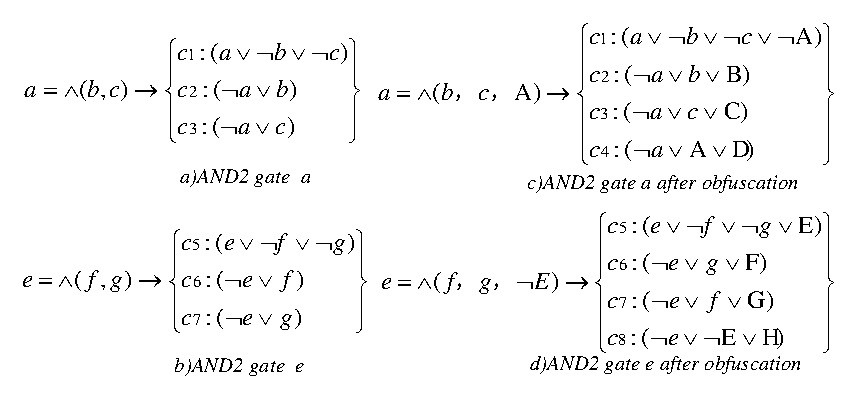
\includegraphics[width=8.2cm]{AND2-2}
%%\caption{CNF signature of $a$ and $e$ before and after obfuscation}
%%\label{4:fig_beforeafter}
%%\end{figure}
%%
%%%Figure \ref{4:fig_beforeafter}a) and \ref{4:fig_beforeafter}b) shows the CNF signature and hyper-graph of two AND2 gate $a$ and $e$.
%%%While their CNF signature and hypergraph after obfuscating are shown in Figure \ref{4:fig_beforeafter}c) and \ref{4:fig_beforeafter}d).
%%Figure \ref{4:fig_beforeafter}a) and \ref{4:fig_beforeafter}b) shows the CNF signatures of two AND2 gates $a$ and $e$,
%%while their CNF signatures after obfuscation are shown in Figure \ref{4:fig_beforeafter}c) and \ref{4:fig_beforeafter}d).
%%
%%There are three types of changes:
%%\begin{enumerate}
%% \item
%% The length of key clauses $c_1$ and $c_5$ are changed from 3 to 4,
%%this defeats structure detection techniques \upcite{csFu} based on key clause oriented pattern matching;
%% \item
%%CNF signatures of $a$ (characteristic clauses $c_1$-$c_3$) and $e$ (characteristic clauses $c_5$-$c_7$) are changed into different forms,
%%and there are new clauses added in formula, such as $c_4$ and $c_8$,
%%This defeats structure detection techniques\upcite{csRoy} based on sub-graph isomorphic;
%%\item
%% By inserting proper literals in key clauses and generating new clause,
%% CNF signature of gate $a$ is changed from AND2 to AND3,
%%shown in Figure \ref{4:fig_beforeafter}a) and \ref{4:fig_beforeafter}c).
%%Husk variable $A$,
%%which becomes an input variable of gate AND3,
%%is indistinguishable with $b$ and $c$,
%%which are original input variables of AND2.
%%This makes it impossible to distinguish gates AND2 and AND3.
%%\end{enumerate}
%
%通过增加冗余的文字和子句,
%OBFUSCATOR可以将CNF公式中的标记改变为另一合法标记.
%在混淆之后,原始的CNF公式就被转化为混有噪音电路的另一个公式。
%由于混淆后的的CNF公式被外包作为SAT求解器的输入,
%原始CNF公式中的电路结构就并不再直接暴露给潜在的攻击者.
%
%\begin{figure}[b]
%\centering
%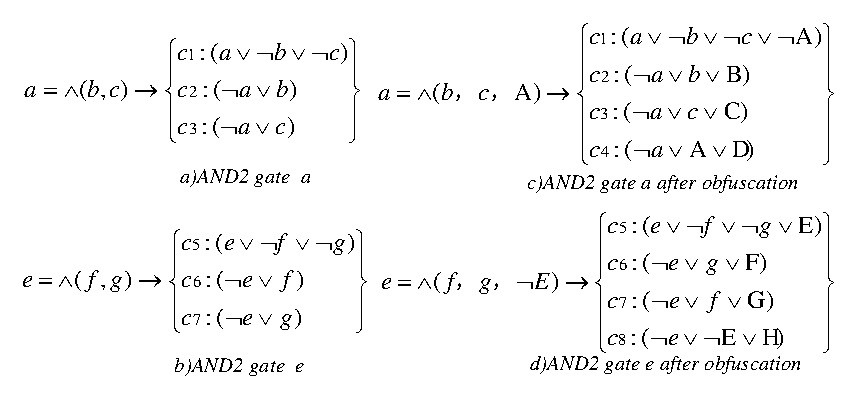
\includegraphics[width=8.2cm]{AND2-2}
%\caption{混淆前后$a$和$e$的CNF标记}
%%\caption{CNF signature of $a$ and $e$ before and after obfuscation}
%\label{4:fig_beforeafter}
%\end{figure}
%
%%Figure \ref{4:fig_beforeafter}a) and \ref{4:fig_beforeafter}b) shows the CNF signature and hyper-graph of two AND2 gate $a$ and $e$.
%%While their CNF signature and hypergraph after obfuscating are shown in Figure \ref{4:fig_beforeafter}c) and \ref{4:fig_beforeafter}d).
%图\ref{4:fig_beforeafter}a) 和\ref{4:fig_beforeafter}b) 给出了两个AND2门$a$和$e$CNF 标记,
%混淆后的标记显示在图\ref{4:fig_beforeafter}c)和\ref{4:fig_beforeafter}d)中.
%
%有三种改变
%\begin{enumerate}
% \item
% 关键子句$c_1$和$c_5$ 的长度由3变为4,
%基于关键子句模式匹配的电路结构探测算法\upcite{csFu}将不再有效;
% \item
%$a$的特征子句$c_1$-$c_3$)以及$e$的特征子句$c_5$-$c_7$变为了不同的形式,
%并且有新的子句加入了公式如$c_4$和$c_8$,
%基于标记子图同构的电路结构检测算法\upcite{csRoy}将不再有效;
%\item
% 通过加入合适的新文字以及构造新的子句,
% 门$a$ 的CNF标记从AND2变为了AND3,
%如图\ref{4:fig_beforeafter}a)和\ref{4:fig_beforeafter}c)。
%Husk文字$A$,
%成为了新生成的AND3门的一个输入,
%并且与原始AND2门的输入$b$和$c$不可区分。
%这也使得区分混淆后AND2和真实AND3变得不再可能.
%\end{enumerate}
%%
%%\subsubsection{Output Camouflage by over-approximating solution space}
%\textbf{输出数据隐藏}
%根据\ref{4:SSOtheorem},
%在SSO obfuscation之后解空间为原解空间的上估计.
%这也就意味着,SAT求解器都无法确切知道真实的解。
%首先,他们无法区分原始公式的变量和Husk公式的变量,而Husk公式的变量的赋值对验证毫无意义。
%其次,他们无法确认一个可满足解也意味着原始SAT问题也是可满足,因为混淆会引入假解。
%通过解空间上估计,我们把一个Rare Events转变为了一个Camouflaged Rare Events,这也是文献\upcite{HV-grid} 曾经期待的事情。
%
%\subsection{算法复杂性评估}
%\textbf{混淆算法的复杂性}
%%Obfuscation is implemented in Algorithm \ref{4:algo_obs}.
%%The main procedure of Algorithm \ref{4:algo_obs} consists only one layer of loop,
%%but one of it sub-procedure $\mathbf{mark}$ (Algorithm \ref{4:algo_mark}) consists 4 layers of loop,
%%and the runtimes of the 2 inner loops are bounded by length of clauses.
%%So the complexity of the obfuscation algorithm is $O(n^2)$.
%算法\ref{4:algo_obs}实现了混淆,其中主程序仅仅包含一层循环,
%但是其中一个子程序$\mathbf{mark}$(算法\ref{4:algo_mark})包含了4层循环,
%由于两层内循环的上界为子句长度,因此混淆算法复杂性为$O(n^2)$。
%\textbf{解恢复算法的复杂性}
%%Solution recovery is implemented in  Algorithm \ref{4:algo_map},
%%which only consists one layer of loop,
%%its complexity is $O(n)$.
%%According to Theorem \ref{4:SSOtheorem}, result from SAT solver may consist false solution,
%%so Algorithm \ref{4:algo_map} may be run more than one time to get correct solution.
%%Since Algorithm \ref{4:algo_map} is of linear complexity,
%%it incurs minor impact on performance of SAT Solving.
%解恢复在算法\ref{4:algo_map}中实现,
%由于仅仅包含一层循环,算法复杂度为$O(n)$.
%根据定理\ref{4:SSOtheorem}, 来自于SAT求解器的解可能包含假解,
%因此为获得正确解,算法\ref{4:algo_map}可能会运行不只一次.
%由于算法\ref{4:algo_map}为线性复杂度,
%带给整个求解过程的开销较小.
%%\section{Related work}
%%\textbf{Secure Computation Outsourcing based on encryption:}
%%R. Gennaro et al.\upcite{R.Gennaro} presented the concept of verifiable computation scheme,
%%which shows the secure computation outsourcing is viable in theory.
%%But the extremely high complexity of FHE operation and the pessimistic circuit sizes make it impractical.
%%Zvika et al.\upcite{OBfuscationd-CNFs} constructed an obfuscated program for d-CNFs that preserves its functionality without revealing anything else.
%%The construction is based on a generic multi-linear group model and graded encoding schemes,
%%along with randomizing sub-assignments to enforce input consistency.
%%But the scheme incurs large overhead caused by their fundamental primitives.
%%
%%\textbf{Secure Computation Outsourcing based on disguising:}
%%For linear algebra algorithms,
%%Atallah et al. \upcite{t19} multiplied data with random diagonal matrix before outsourcing.
%%and recovered results by reversible matrix operations.
%%Paper \upcite{t20} discussed secure outsourcing of numerical and scientific computation,
%%by disguising with a set of problem dependent techniques.
%%C.Wang\upcite{c.WANG} presented securely outsourcing linear programming(LP) in Cloud,
%%by explicitly decomposing LP computation into public LP solvers and private data,
%%and provide a practical mechanism which fulfills input/output privacy,
%%cheating resilience, and efficiency.
%%
%%\textbf{Verifiable computation delegation:}
%%Verifiable computation delegation is the technique to enable
%%a computationally weak customer to verify the correctness of the delegated computation results
%%from a powerful but untrusted server without investing too much resources.
%%To prevent participants from keeping the rare events,
%%Du. et al. \upcite{HV-grid} injected a number of chaff items into the workloads so as to confuse dishonest participants.
%%Golle et al. \upcite{t32} proposed to insert some pre-computed results images of ringers
%%into the computation workload to defeat untrusted or lazy workers.
%%Szada et al. \upcite{t33} extended the ringer scheme and propose methods
%%to deal with cheating detection.
%%
%%\section{相关工作}
%%\textbf{基于加密的安全计算外包:}
%%R. Gennaro等人\upcite{R.Gennaro}给出了可验证计算的策略,
%%指出了安全计算外包的理论上可行性.
%%但是同构加密操作的复杂性和悲观的电路尺寸使得还未能实际使用.
%%Zvika等人\upcite{OBfuscationd-CNFs}构造了面向d-CNFs的混淆程序,用来保持函数功能的同时隐藏信息.
%%他们的构造过程基于通用的多线性群模型以及坡度加密策略,以及随机的赋值以保证输入的一致性。
%%他们的方法是面向通用的SAT 问题,由于原语引入的开销较大。
%%
%%\textbf{基于伪装的安全计算外包:}
%%对于线性代数算法,
%%Atallah等人\upcite{t19}使用对角矩阵乘来伪装外包数据,并通过反向矩阵操作来恢复结果。
%%文献\upcite{t20}讨论了通过特定问题相关技术来伪装数据,实现数值和科学计算的安全外包。
%%C.Wang\upcite{c.WANG}给出了线性规划的安全外包方法,
%%通过显示的将LP计算划分为公共的LP求解和私有数据,
%%并且给出了实现输入输出隐私保护,欺骗防御的可行的机制.
%%
%%\textbf{可验证的计算代理:}
%%可验证计算代理技术是指,一个计算能力弱的客户端可以较小的计算量来验证不可信服务器提供的计算结果正确性。
%%Golle et al. \upcite{t32} 给出了插入预先计算结果到计算负载中,以便于防止不诚实以及懒惰的工人。
%%Szada et al. \upcite{t33} 扩展了ringer策略并且给出了欺骗检测的方法.
%%为了防止不可信的计算参与者持有计算结果,
%%Du等人\upcite{HV-grid}将一定数量的chaff插入到工作集中以便于误导不诚实的参与者.
%%
%%\section{实验评估}
%%%Algorithms presented in this paper are implemented in language $C$.
%%%The experiments is conducted on a laptop with Intel Core(TM) i7-3667U CPU @ 2.00GHz, 8GB RAM.
%%%
%%%We unroll circuits in ISCAS89 benchmark for 100 times and transform them into CNF formulas,
%%%and generate Husks formula with variables number $vn=675$ and clauses number $cn=2309$,
%%%and then obfuscate the CNF formula by transform 2 input gates into 3 input gates.
%%%We use MiniSat as solver.
%%%
%%%Table \ref{4:fig_exp} presents experiments result on benchmarks, meaning of parameters are listed below. \\
%%%$~~$\textbf{vn/cn}:variable and clause number of CNF formula.\\
%%%$~~$\textbf{Marked Gate}:number of gates being changed in obfuscation.\\
%%%$~~$\textbf{Solve Times}:SAT Solver time before and after obfuscation.\\
%%%$~~$\textbf{Obfuscation Times}:obfuscation time.\\
%%%$~~$\textbf{Map Time}:solution recovery time.
%%%
%%%Acccording to Algorithm \ref{4:algo_obs},
%%%Obfusaction time is up to number of gates being changed,
%%%while solution recovery time is up to size of CNF formula,
%%%experiments manifest the fact.
%%%% Detailed information are listed in columns of \textbf{Marked~Gate}, \textbf{Obfuscation Times} and \textbf{Map~Times}.
%%%
%%%As for Asymmetric Speedup\upcite{c.WANG}, for more than 60 \% of circuits, the value is more than 260\%,
%%%It indicates the necessity of outsourcing complex SAT solving.
%%%But for some small size circuits,
%%%Asymmetric Speedup is less than 1.
%%%Especially for circuit s3384,
%%%since the obfuscation takes lots of time to transform 139860 gates, Asymmetric Speedup is only 5.22\%.
%%%\begin{equation}
%%% Asymmetric~Speedup= \frac{Solving~Time}{Obfuscation~Times + Map~Time}
%%%\end{equation}
%%%
%%%The experiments also show that overhead of SAT solving time, incurred by obfuscation,
%%%are different among circuits.
%%%For more than 60 \% of circuits, overhead is less than 30\%; But for the other 40\% circuits, overhead exceed 100\%.
%%%
%%%These facts remind us at least two things:
%%%First, since  obfuscation time is up to gates being changed,
%%%delicate obfuscation algorithm which change less gates but still can mislead adversary should be studied.
%%%Second, since overhead on SAT solving incurred by obfuscation are different among circuit benchmarks,
%%%much more attention should be pay on the impact on solving time,  when designing obfuscation algorithm.
%%%\begin{figure}
%%%\centering
%%%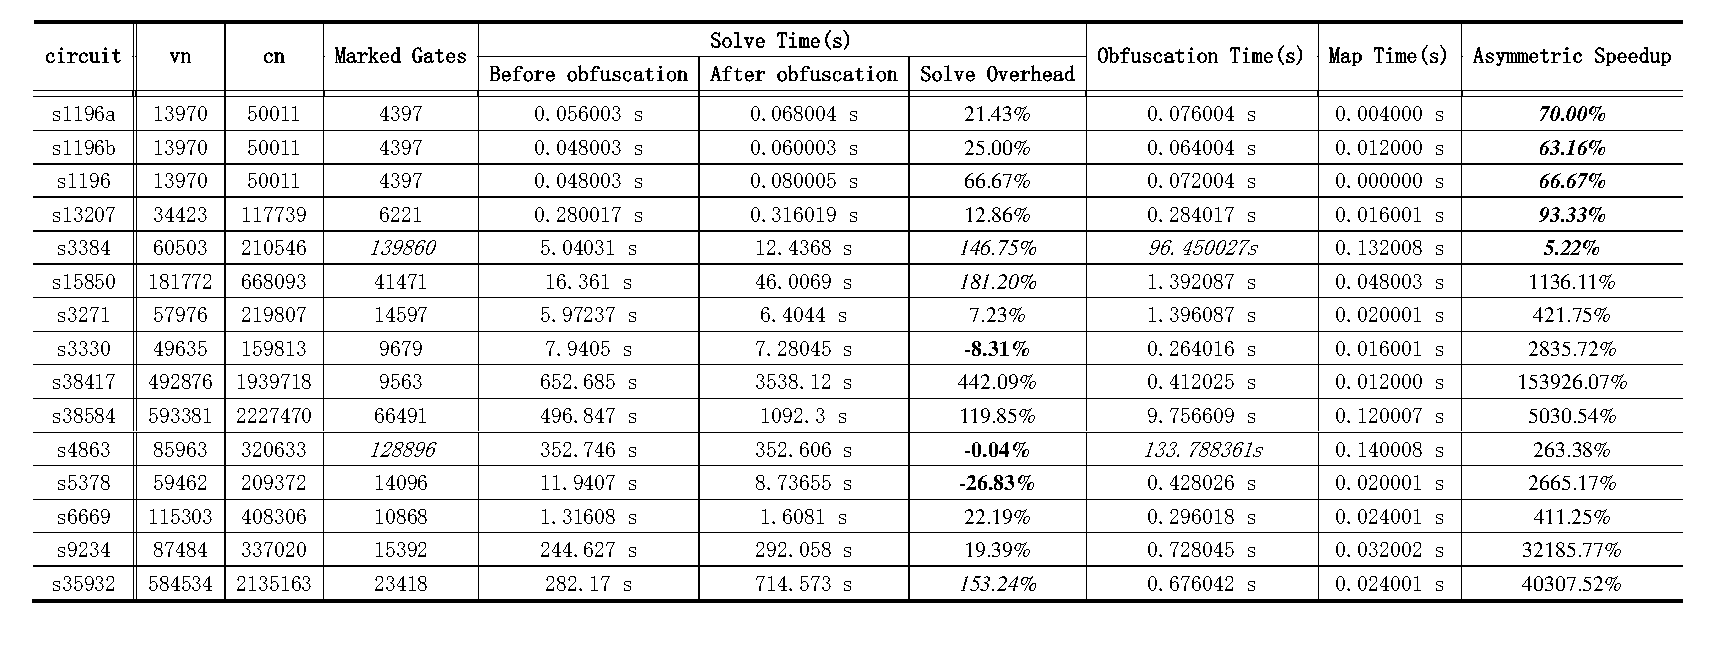
\includegraphics[width=16cm]{Experiment}
%%%\caption{Relationship between Runtime and Size of CNF formula}
%%%\label{4:fig_exp}
%%%\end{figure}
%%\subsection{实验设计}
%%本文给出的算法由C语言实现.
%%实验用机器的配置为Intel Core(TM) i7-3667U CPU @ 2.00GHz, 8GB RAM.
%%
%%将ISCAS89测试集中的部分电路展开100次并编码为CNF公式,
%%产生的Husks公式包含了节点数和子句数为$vn=675$/$cn=2309$,
%%并且将原始公式中的2输入门转换为3输入门.
%%使用MiniSat作为求解器.
%%
%%\subsection{实验结果分析}
%%表\ref{4:fig_exp}给出了实验结果,表中各个参数的意义如下所示。 \\
%%$~~$\textbf{vn/cn}:CNF 公式中的变量数和子句数.\\
%%$~~$\textbf{Marked Gate}: 混淆过程中改变的门数.\\
%%$~~$\textbf{Solve Times}: 混淆前后的SAT求解时间.\\
%%$~~$\textbf{Obfuscation Times}:混淆时间.\\
%%$~~$\textbf{Map Time}:解恢复时间.
%%
%%根据算法\ref{4:algo_obs},
%%混淆时间取决于改变的门数,
%%解恢复时间取决于CNF公式的尺寸,
%%实验表明了这一事实.
%%% Detailed information are listed in columns of \textbf{Marked~Gate}, \textbf{Obfuscation Times} and \textbf{Map~Times}.
%%
%%就异构加速比( Asymmetric~Speedup)\upcite{c.WANG}而言,60\%的电路, 值超过了260\%,
%%这表明了外包复杂SAT求解函数的必要性.
%%某些尺寸较小的电路B,异构加速比小于1.
%%特别是对于电路s3384,
%%由于混淆花费了大量的时间,转换了139860个门,使得异构加速比仅为5.22\%.
%%\begin{equation}
%% Asymmetric~Speedup= \frac{Solving~Time}{Obfuscation~Times + Map~Time}
%%\end{equation}
%%
%%实验也显示出SAT求解的开销,不同的电路具有不同的表现。
%%60 \% 以上的电路,开销小于30\%;而40\%电路,开销超过了100\%.
%%
%%这些事实提醒我们两件事情:
%%首先,混淆时间取决于被改变的门数,
%%需要研究更加精巧的混淆算法以改变较少的门的情况下仍然可以迷惑攻击者.
%%第二, 由于混淆引入的SAT求解开销,因电路而异,在设计混淆算法时,需要考虑修改后结构对求解时间的影响。
%%
%%\begin{table*}
%%\caption{不同类型电路的CNF 公式的运行时间}
%%%\caption{Runtime of CNF formula generated from different Circuit}
%%\centering
%%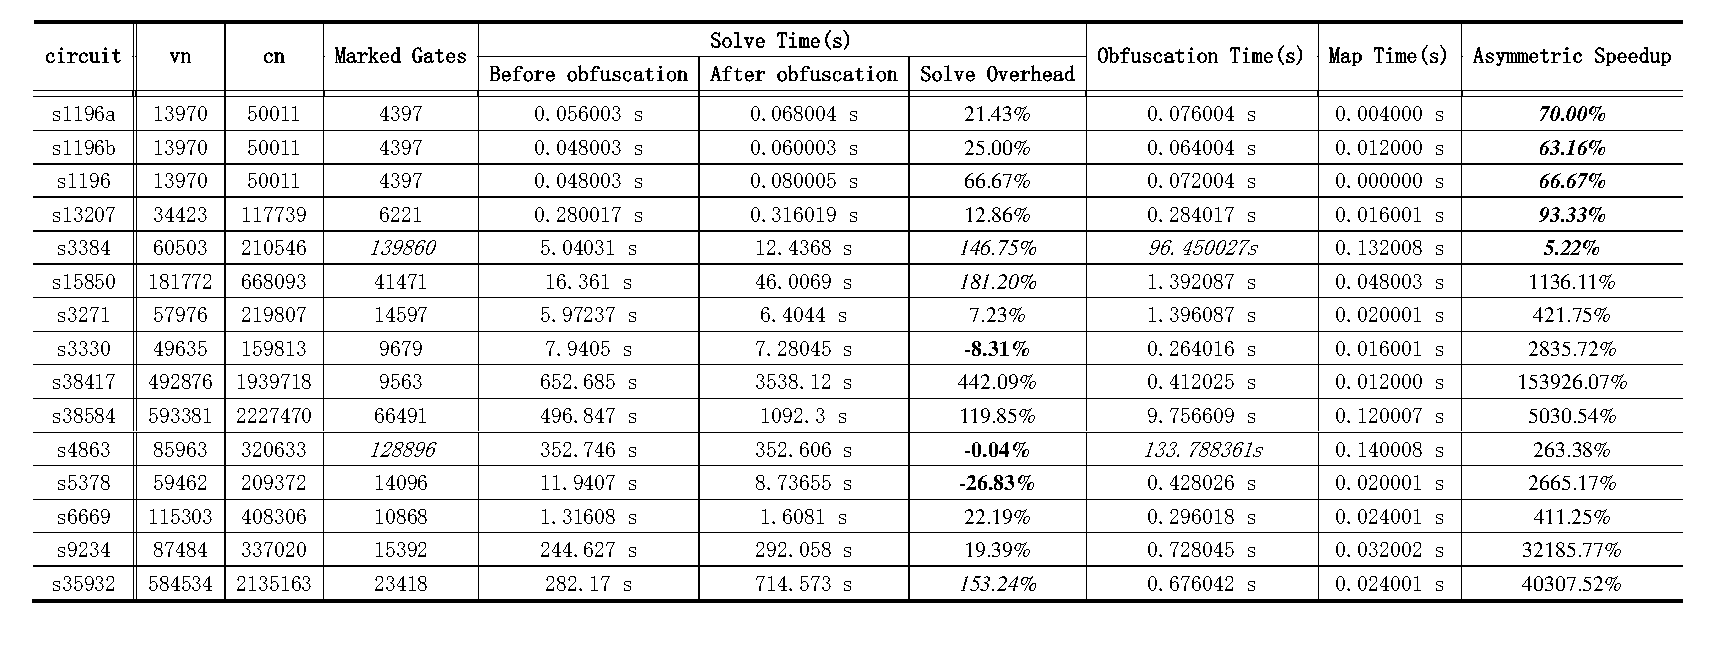
\includegraphics[width=12.2cm]{Experiment}
%%\label{4:fig_exp}
%%\end{table*}%
%%
%%\section{Conclusion}
%%This paper proposes a circuit aware  CNF obfuscation algorithm,
%%that can prevent the confidential information from being recovered by adversary,
%%when outsourcing SAT problem in Cloud or grid.
%%Theoretical analysis and experimental results show that algorithms can significantly change structure of CNF formula,
%%with polynomial complexity and without narrowing down its solution space.
\section{本章小结}
本文给出了电路结构感知的CNF 混淆算法,可防止在SAT问题外包计算时,CNF公式中的电路结构以及解被窃取。
理论分析表明,算法可以有效的改变结构,同时还将扩展CNF公式的解空间。
